\documentclass[12pt,twoside=off,
bibliography=totoc,
listof=totoc,appendixprefix,paper=a4,headings=small]{scrbook} % 'twoside=on' für Druckversion oder 'twoside=off' für Onlineversion

%
% Packages
% -----------------------------------
\usepackage[
  paper=a4paper,
  left=12.5mm,
  right=25mm,
  top=25mm,
  bottom=50mm,
  bindingoffset=10mm]{geometry}		% Seitenränder und Bindungskorrektur einstellen
  
\usepackage{apacite} 				% Literatur-Referenzen: American Psycholog. Assoc.
\usepackage{natbib}					

\setcitestyle{round,aysep={}} 		% Indizierg. in runden Klammern, zw. Autor u. Jahr
\usepackage[utf8]{inputenc}         % Umlaute im Text
\usepackage{ngerman}				% Rechtschreibg.
\usepackage[T1]{fontenc}
\usepackage{lmodern}				% Schriftfamilie
\usepackage{microtype}				% für die Mikrotypografie (besseres Schriftbild)

\usepackage{graphicx} 				% Grafiken einfügen (pdf,png - aber jpg vermeiden)
\graphicspath{{./Bilder/}}          % Pfad zu den Bildern

\usepackage{url}					% URL's formatieren (z.B. in Literatur) 
\usepackage[colorlinks,linkcolor=black,citecolor=black,urlcolor=black]{hyperref} 				% für Hyperlinks in PDF-Dokumenten   
  
\usepackage{tabularx} 				% bessere Gestaltung von Tabellen
\usepackage{longtable} 		
\usepackage{multicol}				
\usepackage{multirow}
\usepackage{booktabs}
\usepackage{tabularx}
		
\usepackage[active]{srcltx}

\usepackage{graphicx} % Für \resizebox
\usepackage{tikz}     % Für TikZ-Grafiken
\usetikzlibrary{
    positioning,      % Für below=of, right=of, left=of
    shapes.geometric, % Für diamond und geometrische Formen
    arrows.meta       % Für >=Stealth
}

\usepackage{listings}
\usepackage{algorithm}
\usepackage{algpseudocode}				% Algorithmen

\usepackage{mdwlist}				% Listen

\usepackage{setspace} 				% Zeileneinstellung
\newtheorem{mydef}{Merksatz}  		% Falls Beispiele, Merksätze m. fortl. Nr. gebr. werden
\newtheorem{bsp}{Beispiel}

\usepackage{todonotes}				% zum Erstellen von ToDos im Editor

\usepackage{lscape}					% zum Rotieren von Seiten

\usepackage{amsmath}				% zum Schreiben von mathematischen Formeln

\usepackage{calc}

\usepackage{footnote}				% Fußnoten
\usepackage{tablefootnote}			% Fußnoten in Tabellen

\usepackage{algorithm}
\usepackage{algpseudocode}

\makeatletter
\newenvironment{breakablealgorithm}
  {%
    \begin{center}
      \refstepcounter{algorithm}%
      \hrule height .8pt depth 0pt \kern 2pt
      \renewcommand{\caption}[2][\relax]{%
        {\raggedright\textbf{\fname@algorithm~\thealgorithm}%
        ##2\par}%
        \kern 2pt\hrule\kern 2pt
      }%
  }
  {%
      \kern 2pt\hrule
    \end{center}
  }
\makeatother

%\clubpenalty = 10000
%\widowpenalty = 10000 \displaywidowpenalty = 10000

\hyphenation{voll-st\"andigen}		% Worttrennungen global definieren

\setcounter{tocdepth}{1}			% Ebenen, die im Inhaltsverzeichnis angezeigt werden

% Document
% -----------------------------------
\begin{document}

\frontmatter 
    % Titelseite soll keine Kopf oder Fußzeile haben
\thispagestyle{empty}

% Alle Elemente sollen zentriert sein
\begin{center}

\vspace*{-10mm}

{\LARGE Wirtschaftsinformatik, \\insb. 
KI-basierte Anwendungssysteme\\[1mm]}

\vspace*{1cm}


\includegraphics[width=0.18\textwidth]{Bilder/up_logo.png}

\vspace*{1cm}

% Art der Arbeit => (Bachelorarbeit ,Diplomarbeit, Masterarbeit, Seminararbeit)
{\Large \textbf{Masterarbeit}}\\ 

\vspace{1cm}

% Titel der Arbeit 
{\large \textbf{Traumasensible KI-Chatbots im Coaching}}\\ 

\vspace{1.5cm}

% Name des/der Autors/Autoren
{\LARGE Julia Jellinek}\\[15mm]

% Gutachter, Kontaktdaten und Abgabetermin
\parbox{120mm}{
\begin{large}
\begin{tabbing}
Gutachter(in): \hspace{.7cm} \=Prof. Dr.-Ing. Marcus Grum\\[4mm]
Semester:\> Sommersemester 2026\\
Verfasser:\> Julia Jellinek\\ % alphabetische Reihenfolge (Nachname)
Matrikel-Nr.:\> 825812\\
Adresse:\> Eva-Laube-Weg 1, 14473 Potsdam\\
Email:\> julia.jellinek@uni-potsdam.de\\
Telefon:\>015251304477\\
Studienfach:\>Wirtschaftsinformatik und digitale Transformation\\[8mm]
\textbf{Abgabetermin:} \> \textbf{27. November 2026}\\
\end{tabbing}
\end{large}
}

\end{center}
\clearpage{\pagestyle{empty}\cleardoublepage}
 			% Titelblatt
    \thispagestyle{empty}

\vspace*{1cm}

\begin{center}
    \textbf{Abstract}
\end{center}

\vspace*{1cm}

\noindent 
Dieser Blindtext zeigt den ungefähren Umfang des deutschen Abstract.Lorem ipsum dolor sit amet, consectetuer adipiscing elit. Aenean commodo ligula eget dolor. Aenean massa. Cum sociis natoque penatibus et magnis dis parturient montes, nascetur ridiculus mus. Donec quam felis, ultricies nec, pellentesque eu, pretium quis, sem. Nulla consequat massa quis enim. Donec pede justo, fringilla vel, aliquet nec, vulputate eget, arcu. In enim justo, rhoncus ut, imperdiet a, venenatis vitae, justo. Nullam dictum felis eu pede mollis pretium. Integer tincidunt. Cras dapibus. Vivamus elementum semper nisi. Aenean vulputate eleifend tellus. Aenean leo ligula, porttitor eu, consequat vitae, eleifend ac, enim. Aliquam lorem ante, dapibus in, viverra quis, feugiat a, tellus. Phasellus viverra nulla ut metus varius laoreet. Quisque rutrum. Aenean imperdiet. Etiam ultricies nisi vel augue. Curabitur ullamcorper ultricies nisi. Nam eget dui. Etiam rhoncus. Maecenas tempus, tellus eget condimentum rhoncus, sem quam semper libero, sit amet adipiscing sem neque sed ipsum. Nam quam nunc, blandit vel, luctus pulvinar, hendrerit id, lorem. Maecenas nec odio et ante tincidunt tempus. Donec vitae sapien ut libero venenatis faucibus. Nullam quis ante. Etiam sit amet orci eget eros faucibus tincidunt. Duis leo. Sed fringilla mauris sit amet nibh. Donec sodales sagittis magna. Sed consequat, leo eget bibendum sodales, augue velit cursus nunc, quis gravida magna mi a libero. Fusce vulputate eleifend sapien. Vestibulum purus quam, scelerisque ut, mollis sed, nonummy id, metus. Nullam accumsan lorem in dui. Cras ultricies mi eu turpis hendrerit fringilla. Vestibulum ante ipsum primis in faucibus orci luctus et ultrices posuere cubilia Curae; In ac dui quis mi consectetuer lacinia. Nam pretium turpis et arcu. Duis arcu tortor, suscipit eget, imperdiet nec, imperdiet iaculis, ipsum.

 	% Abstract auf Deutsch 
    \newpage
    \clearpage{\pagestyle{empty}\cleardoublepage}
    \thispagestyle{empty}


\vspace*{1cm}

\begin{center}
    \textbf{Abstract}
\end{center}

\vspace*{1cm}

\noindent 
The following blindtext illustrates the length of the Abstract in english. Lorem ipsum dolor sit amet, consectetuer adipiscing elit. Aenean commodo ligula eget dolor. Aenean massa. Cum sociis natoque penatibus et magnis dis parturient montes, nascetur ridiculus mus. Donec quam felis, ultricies nec, pellentesque eu, pretium quis, sem. Nulla consequat massa quis enim. Donec pede justo, fringilla vel, aliquet nec, vulputate eget, arcu. In enim justo, rhoncus ut, imperdiet a, venenatis vitae, justo. Nullam dictum felis eu pede mollis pretium. Integer tincidunt. Cras dapibus. Vivamus elementum semper nisi. Aenean vulputate eleifend tellus. Aenean leo ligula, porttitor eu, consequat vitae, eleifend ac, enim. Aliquam lorem ante, dapibus in, viverra quis, feugiat a, tellus. Phasellus viverra nulla ut metus varius laoreet. Quisque rutrum. Aenean imperdiet. Etiam ultricies nisi vel augue. Curabitur ullamcorper ultricies nisi. Nam eget dui. Etiam rhoncus. Maecenas tempus, tellus eget condimentum rhoncus, sem quam semper libero, sit amet adipiscing sem neque sed ipsum. Nam quam nunc, blandit vel, luctus pulvinar, hendrerit id, lorem. Maecenas nec odio et ante tincidunt tempus. Donec vitae sapien ut libero venenatis faucibus. Nullam quis ante. Etiam sit amet orci eget eros faucibus tincidunt. Duis leo. Sed fringilla mauris sit amet nibh. Donec sodales sagittis magna. Sed consequat, leo eget bibendum sodales, augue velit cursus nunc, quis gravida magna mi a libero. Fusce vulputate eleifend sapien. Vestibulum purus quam, scelerisque ut, mollis sed, nonummy id, metus. Nullam accumsan lorem in dui. Cras ultricies mi eu turpis hendrerit fringilla. Vestibulum ante ipsum primis in faucibus orci luctus et ultrices posuere cubilia Curae; In ac dui quis mi consectetuer lacinia. Nam pretium turpis et arcu. Duis arcu tortor, suscipit eget, imperdiet nec, imperdiet iaculis, ipsum.
    \newpage
    
    \clearpage{\pagestyle{empty}\cleardoublepage}
    \thispagestyle{empty}


\vspace*{1cm}

\begin{center}
    \textbf{Sperrvermerk}
\end{center}

\vspace*{1cm}

\noindent 

Die vorgelegte Masterarbeit basiert auf internen, vertraulichen Daten und Informationen des Unternehmens ...... In diese Arbeit dürfen Dritte, mit Ausnahme der Gutachter und befugten Mitgliedern des Prüfungsausschusses ohne ausdrückliche Zustimmung des Unternehmens und des Verfassers keine Einsicht nehmen. Von diesem Verbot ausgenommen sind außerdem jene Personen, die auch ansonsten zur Einsichtnahme in die genannten Daten und Informationen befugt sind. Eine Vervielfältigung und Veröffentlichung der Masterarbeit ohne ausdrückliche Genehmigung – auch auszugsweise – ist nicht erlaubt.

\vspace{2cm}

\noindent
Berlin, den 01. Januar 2099

\vspace{3cm}

\hspace*{7cm}%
\dotfill\\
\hspace*{8.5cm}%
\textit{(Unterschrift des Verfassers)}      % Sperrvermerk
    \newpage
    
    \clearpage{\pagestyle{empty}\cleardoublepage}
    \onehalfspacing                  	% Zeilenabstand ab hier 1.5 zeilig
    \tableofcontents 					% Inhaltsverzeichnis
    \clearpage{\pagestyle{empty}\cleardoublepage} 
    
    \listoffigures 					 	% Abbildungsverzeichnis
    \clearpage{\pagestyle{empty}\cleardoublepage}
    
    \listoftables						% Tabellenverzeichnis
    \clearpage{\pagestyle{empty}\cleardoublepage}

% -----------------------------------
\mainmatter 							% die einzelnen Kapitel
    \chapter{Einleitung}

Die letzten Jahre haben gezeigt, dass künstliche Intelligenz (KI) und insbesondere Chatbots
zunehmend Einzug in den Coaching-Sektor hatten und als digitale Selbstcoaching-Tools
betrachtet werden \citep{mai2023chatbots}. KI stellt eine Schnittmengen zur Datenwissenschaft dar, wobei durch den Einsatz von Techniken und Systemen intelligentes Verhaltens erzeugt wird\citep{balzert2009software}. 
Ein KI-gestützter Chatbot ist eine Softwareanwendung, die auf künstlicher Intelligenz basiert und mittels natürlicher Sprache mit Menschen kommuniziert. 
Sie werden als Large Language Models (LLMs) bezeichnet. Dabei handelt es sich um KI-Modelle, die auf der Verarbeitung und Erzeugung von natürlicher Sprache
basieren. Sie nutzen riesige Mengen an Textdaten, um statistische Muster zu lernen und
darauf basierend Outputs zu generieren \citep{Douglas2023Large}.
Als Designmerkmale werden gestaltungsbezogene Eigenschaften eines LLM Systems verstanden. Um abzuleiten, welche Ausprägung Designmerkmale haben müssen,
wird das Verständnis vom Anthropomorphismus betrachtet. Dies ist ein wechselseitiges Phänomen, bei dem Designer menschenähnliche Merkmale in Artefakte einbetten und die Betrachter ihre kognitive Reaktion auf diese Merkmale auf die Artefakte projizieren \citep{Xiao2025Humanizing}. Interaktionsmerkmale von Sprachmodellen sind die Eigenschaften der Mensch Modell Interaktion, die sich in der Gestalt der Prompts ausdrücken – also wie Aufgaben als Anweisungen formuliert, strukturiert und iterativ verfeinert werden, um das gewünschtes Verhalten des Modells zu erreichen. Ein Prompt ist eine natürliche Sprachinstruktion, mit der der Mensch das Modell steuert \citep{Gao2023Prompt}. 
Der Begriff Coaching bezeichnet eine zeitlich begrenzte, interaktive Begleitung, bei der Coaches Klienten dabei unterstützen, persönliche oder berufliche Ziele eigenverantwortlich zu definieren und zu erreichen. Der sprachliche Ursprung liegt im ungarischen Wort „kocsi“ (Kutsche) als Metapher für ein Beförderungsmittel ans gewünschte Ziel \citep{sonesh2015power, nyfoudi2021talent}.
Coaching hat sich in verschiedenen Praxisfeldern als personenorientiertes Beratungsformat etabliert, das die Selbststeuerung und
persönliche Entwicklung von Einzelpersonen, Teams und Organisationen unterstützt. Neben
klassischen Präsenzformaten gewinnen digitale Coaching-Formate, wie E-Mail-, Chat- oder
VR-Coaching, zunehmend an Bedeutung \citep{strong2020chatbots}. 
Das wesentliche Merkmal von VR ist die Inklusion, dass heißt, das Umgeben-Sein von einer Umgebung. VR versetzt den Teilnehmenden mitten in Informationen hinein \citep{bricken1990learning}. 
Vorwiegend KI gestützte Chatbots werden eingesetzt, um Soft Skills zu trainieren oder Reflexionsprozesse
zu unterstützen \citep{mai2020ai}. Softskills sind überfachlichen verhaltens- und beziehungsbezogenen sowie emotionale und kognitive Kompetenzen \citep{dell2017educational, werning2023virtual}.

\section{Problemstellung}

Im Jahr 2021 waren über 46,7 Millionen amerikanische Erwachsene von psychischen Erkrankungen betroffen, wobei nur 41,3\% im Laufe des Jahres eine psychotherapeutische
Behandlung erhielten. Mehr als 60\% derjenigen, die im Vorjahr behandelt wurden,
gaben an, virtuelle Angebote in Anspruch genommen zu haben. Als hinderliche Gründe psychotherapeutischer Behandlungen werden Kosten, Zeitaufwand, Unwissenheit über Anlaufstellen und die Annahme, die Probleme
selbst bewältigen zu können herausgestellt. Es besteht ein Zusammenhang zwischen psychischen Erkrankungen, der Inanspruchnahme von Behandlungen und einem
wahrgenommenen ungedeckten Bedarf an Versorgung \citep{Forman-Hoffman2025Prevalence}.
Trotz der wachsenden Verbreitung von Coaching-Chatbots bleibt unklar, in
welchem Umfang diese menschliche Therapie oder Coaching ersetzen können, insbesondere
in sensiblen Kontexten wie der Traumaarbeit. Im Folgenden wird der Begriff Trauma nach
dem Verständnis von \cite{Levine2010}  verwendet, da im Rahmen dieser Arbeit nicht die
klinische Diagnostik, sondern eine traumasensible Ausrichtung im Coaching-Kontext im
Vordergrund steht. Demnach wird Trauma nicht als Störung, sondern eine Verletzung,
verursacht durch Angst, Hilflosigkeit und Verlust verstanden. Levine beschreibt die damit
verbundene angeborene Fähigkeit zur Heilung durch Selbstregulation von Erregungszuständen und intensiven Emotionen. Traumasensibles Coaching ist demnach darauf ausgerichtet,
selbstregulatorische Prozesse zu unterstützen. Daraus ergeben sich zentrale Erfolgsfaktoren menschlichen Coachings wie Empathie, Wertschätzung und Vertrauen. Diese sind bislang nur begrenzt auf
die Mensch-Maschine-Interaktion übertragbar \citep{mai2020ai}.  Es bestehen ethische Bedenken und Risiken hinsichtlich fehlender emotionaler Sicherheit, unzureichender und unklarer Verantwortlichkeiten \citep{passmore2023can}.

\section{Zielsetzung}

Ein großes Thema bei der Entwicklung erfolgreicher Sprachmodelle ist, sich mit der Personalisierung dieser zu beschäftigen, um Interaktionen, Inhalte und Empfehlungen an die
individuellen Nutzerpräferenzen anzupassen \citep{Tan2024}. Bezüglich der Anwendung von LLMs im therapeutischen oder Coaching Kontext kann dies jedoch bedeuten, das individuelle, nicht entwicklungsfördernde Muster von Klienten vom System adaptiert werden \citep{Xiao2025Humanizing}.
Ziel der Arbeit ist es, ein theoretisch fundiertes Modell für ein KI-gestütztes
Coaching-System zu entwickeln, das auf einer klar definierten Entscheidungslogik beruht. Im
Zentrum steht die Übertragung psychologischer und neurobiologischer Wirkmechanismen
auf künstliche intelligente Systeme. Dabei soll aufgezeigt werden, wie dialogische KI gestaltet
werden kann, dass sie nicht lediglich bestehende Denk- und Verhaltensmuster reproduziert,
sondern zur aktiven Infragestellung und potenziellen Transformation dieser Muster beiträgt,
um auf diese Weise Entwicklungsprozesse zur Traumaheilung der Klienten voranzubringen.
Unter dialogischer KI werden Dialogsysteme verstanden, die über natürliche Sprache mit
Nutzenden interagieren und dabei nicht nur reaktiv auf Eingaben antworten, sondern durch
proaktive Impulse den Gesprächsverlauf aktiv mitgestalten. Dadurch können sie gezielt
Reflexionsprozesse anstoßen und Veränderung unterstützen \citep{Deng2025Proactive}. Die Untersuchung ist besonders relevant, da die zunehmende Digitalisierung der Coachingpraxis
neue Chancen, aber auch Herausforderungen für die professionelle Beratung und ethische
Standards birgt \citep{mai2023chatbots,passmore2023can}.



\section{Forschungsfrage}

\begin{quote}
Welche Design- und Interaktionsmerkmale sind erforderlich, damit ein KI-basierter Chatbot im Coaching-Kontext eine traumasensible Unterstützung zum Prozess der Traumaüberwindung für Personen mit leichten bis moderaten psychischen Belastungen gewährleisten kann?
\end{quote}

\subsection{Einordnung in bisherige Forschung}
Grundlage der Arbeit ist ein theoretisch-konzeptioneller Forschungsansatz, mit dem Ziel, ein strukturbasiertes Modell für den Einsatz von KI-gestützten Chatbots im Coachingkontext zu entwickeln. Ausgangspunkt ist somit einerseits fundiertes Wissen über die Funktionsweisen und Entwicklung künstlicher Intelligenz, insbesondere KI-basierter Sprachmodelle, sowie die Betrachtung psychologischer Theorien. 
Die Persönlichkeits-System-Interaktionen Theorie (PSI) von \cite{Kuhl2000The} erklärt motivationale und willentliche Phänomene wie Konzentration, den Umgang mit Misserfolgen, intrinsische Bindung an persönliche Ziele, Beharrlichkeit und die Umsetzung von Intentionen. Es werden Interaktionsmuster zwischen vier kognitiven Systemen – Denken und Intentionsgedächtnis, Fühlen und Erweiterungsgedächtnis, diskrepanzsensitive Objekterkennung und intuitive Verhaltenskontrolle – durch affektive Veränderungen moduliert. Dies äußert sich in einer veränderten Aktivierung der kognitiven Systeme und damit in beobachtbaren Veränderungen von Selbstregulation, kognitivem Fokus und Handlungsfähigkeit. Dabei unterstützen selbstregulatorische Fähigkeiten affektive Veränderungen beim Lernen und in der Therapie, während entwicklungsbedingte und erzieherische Risikofaktoren diese beeinträchtigen können. Menschliches Verhalten wird nicht von einzelnen Eigenschaften, sondern der Interaktion mehrerer psychischer Systeme beeinflusst. Die PSI-Theorie soll als neurobiologischer Ansatz die Grundlage des betrachteten Problems darstellen. 
Der Anwendungsrahmen der Arbeit bezieht sich auf Coachingprozesse im Kontext leichter bis mittelschwerer psychischer Belastungen bzw. stabiler, aber dysfunktionaler Verhaltensmuster. Leichte Belastungen sind durch milde, vorübergehende Symptome gekennzeichnet, während moderate Belastungen anhaltende und intensivere emotionale Reaktionen hervorrufen, ohne jedoch zu einer schweren Funktionsbeeinträchtigung zu führen. Leichte bis moderate Belastungen können physiologische und psychologische Veränderungen verursachen, die jedoch noch nicht das Ausmaß erreichen, das eine klinische Störung oder akute Gefährdung darstellt \citep{Ovsiannikova2024Peculiarities}.  
Ausgehend von diesem Ansatz untersucht die Arbeit:

    \begin{itemize}
    \item Wie Prompts gestaltet sein müssen, um diagnostisch und reflexionsfördernd zu wirken
  \item Welche Steuerungsmechanismen notwendig sind, um gezielt unterschiedliche psychische Systeme im Sinne der PSI-Theorie zu aktivieren
  \item Welche Risiken bei der Nutzung von KI-Sprachmodellen im traumasensiblen Coaching-Kontext existieren
    \end{itemize}

Zusammenfassend soll die Arbeit herausstellen, wie sich zentrale Mechanismen der PSI-Theorie in konkrete Design- und Interaktionsmerkmale eines KI-basierten Chatbots überführen lassen. 

\section{Aufbau der Arbeit}




    \clearpage{\pagestyle{empty}\cleardoublepage}		% löscht Kopfzeilen und Seitennummerierung von der letzten Seite eines Kapitels, sofern dort kein Text mehr steht
    \chapter{Theoretische Fundierung von KI-gestützten Chatbots im Coaching} \label{chap:2}
Künstliche Intelligenz (KI) ist ein multidisziplinäres Forschungsgebiet, mit Fokus auf der Entwicklung intelligenter Maschinen, die in der Lage sind, Aufgaben zu bewältigen, die normalerweise menschliche Intelligenz erfordern \citep{Sangeetha2023Introduction}. Dazu gehören Aufgaben wie Problemlösung, Entscheidungsfindung, Lernen und das Verstehen natürlicher Sprache. Die KI verfolgt das Ziel, Systeme zu schaffen, die menschliche kognitive Fähigkeiten nachahmen oder replizieren können. Maschinelles Lernen als Teilgebiet der  künstlichen Intelligenz betrachtet die Entwicklung von Algorithmen und statistischen Modellen. Diese befähigen Maschinen auf der Grundlage von Daten zu Lernen und Entscheidungen zu treffen, sowie Vorhersagen zu machen. Deep Leraning meint in diesem Zusammenhang die Anwendung vielschichtiger neuronaler Netze, um aus den unterschiedlichen Abstraktionsebenen der Daten zu lernen.


Ein KI-basiertes Anwendungssystem unterstützt den Anwender dabei, fachliche Aufgaben auf der Grundlage von KI, sowie des Einsatzes von Hardware, Software, sowie möglicherweise logischen Elementen \citep{grum2022construction}. Der Nutzer verwendet die Ergebnisse des KI-basierten Systems und liefert gleichzeitig Daten, die wiederum von dem System genutzt werden.
Chatbots sind KI-basierte Sprachmodelle. Ihre Anwendung und Funktionsweise wird im Folgenden erläutert.

\section{Funktionsweisen von Sprachmodellen}
Unter Natural Language Processing (NLP) versteht man einen Prozess, bei dem Computer menschliche Sprache verstehen, interpretieren und generieren \citep{Sangeetha2023Introduction}. Dies beinhaltet Aufgaben wie Spracherkennung, Sentiment-Analyse, Sprachübersetzung und die Beantwortung von Fragen. 

Large Language Models (LLMs) stellen ein Teilbereich des NLP und damit der künstlichen Intelligenz \citep{Raiaan2024A}. Dies sind Modelle zur Verarbeitung und Generierung natürlicher Sprache. Der Fokus liegt auf dem Training großer Mengen an Textdaten mit dem Ziel, die Bedeutung von Zusammenhängen zu erlernen. Ausgereifte LLMs verfügen über eine Vielzahl von Fähigkeiten, darunter die Generierung, Informationsgewinnung und Zusammenfassung von Texten, sowie die Beantwortung von Fragen, Übersetzung von Sprache, Unterstützung bei Dialogen und Konversationen und das Erzeugen von kontextbezogenen Antworten. Statistische Muster werden genutzt, um Informationen für Vorhersagen nutzbar zu machen. Das bedeutet, getätigte Eingaben werden datenbasiert verarbeitet. Es besteht die Möglichkeit, komplexe sprachliche Strukturen zu erkennen und diese nachzubilden. 

\subsection{Technische Grundlagen von LLMs}
LLMs basieren überwiegend auf der Transformer-Architektur \citep{vaswani2017attention}. Sie zeichnen sich durch eine hohe Skalierbarkeit, parallele und effiziente Verarbeitung langer Texte, sowie einer guten Erfassung von Kontextinformationen aus. 

Zur Verarbeitung der Texte werden diese in einzelne Tokens zerlegt werden \citep{grum2022construction, vaswani2017attention}. Diese sind zum Beispiel Wörter oder einzelne Wortbestandteile, sowie Zeichen oder Symbole. Dann erfolgt die Umwandlung der natürlichen Sprache in maschinenlesbare Einheiten. Diese numerische Darstellung der Tokens als Vektoren wird als Embedding bezeichnet und ermöglicht eine mathematische Verarbeitung der Sprache. Wörter, die eine ähnliche Bedeutung haben liegen im Vektorraum nahe beieinander. Das Konzept des Positional Encoding sorgt in diesem Zusammenhang dafür, ein Verständnis von Satzstruktur und Wortfolge beizubehalten. Besonderes relevante Informationen werden für die gewollte Ausgabe gewichtet. Es werden drei Arten der Attention unterschieden. Self-Attention betrachtet die Beziehungen innerhalb derselben Eingabesequenz, Cross-Attention stellt eine Verknüpfung von Encoder- und Decoder-Informationen bereit und die Full Attention schließlich eine vollständige Berücksichtigung aller Tokens. Der Encoder verarbeitet die Eingabesequenz und wandelt sie in eine mathematische Repräsentation um, die Informationen über die Bedeutung der einzelnen Tokens und ihre Beziehungen zueinander enthält. Durch Decoding wird schließlich eine Ausgabesequenz generiert, welche auf Grundlage der bisher verwendeten Tokens, schrittweise das nächste Token voraussagt. Ausgewählt werden je Folgetokens mit höchster Wahrscheinlichkeit.

Das Training von LLMs basiert auf großen Mengen an Textdaten \citep{Raiaan2024A}. Beim Pre-Training findet ein Lernen allgemeiner Sprachmuster und Wissensrepräsentationen statt. Typische Trainingsdaten stammen aus Webseiten, Büchern oder wissenschaftlichen Texten. Die Erkenntnisse werden anschließend zur Anpassung an spezifische Aufgaben durch Finetuning genutzt. Das vortrainierte Modell wird an spezifische Aufgaben angepasst. Dafür werden kleinere und kontextrelevante Datensätze verwendet. Für den Trainingsprozess ist eine qualitative Datenaufbereitung von Bedeutung. Dies beinhaltet die Entfernung fehlerhafter oder irrelevanter, sowie doppelter Daten und die Exklusion personenbezogener Informationen. Normalisierung ermöglicht anschließend die Stabilisierung des Trainingsprozesses und ermöglicht das Lernen komplexer Muster. Das Verfahren zeichnet sich durch hohen Rechenaufwand und Speicherbedarf, sowie lange Trainingszeiten aus.

\subsection{Neuronale Netzwerke und neuronale Modelle}
Künstliche neuronale Netzwerke (Artificial Neural Networks, ANN) sind rechnergestützte Modelle \citep{grum2022construction,nielsen2015neural,kinnebrock2018neuronale}. Sie orientieren sich an der Struktur und Funktionsweise biologischer Nervensysteme. Diese bestehen aus miteinander verbundenen künstlichen Neuronen, die Informationen verarbeiten und durch Anpassung ihrer Verbindungsgewichte Muster und Zusammenhänge aus Daten erlernen können. 
Neuronale Modellierung basiert auf der mathematischen oder computergestützten Darstellung von Systemen, die sich an der Funktionsweise von biologischen Nervenzellen orientieren. Auf diese Weise werden Prinzipien der Neurowissenschaft, Mathematik und Informatik vereint, um ein Verständnis darüber zu schaffen, wie ein System auf Basis von Neuronen funktioniert und wie diese miteinander interagieren. Ziel des Konzeptes neuronaler Modellierung ist es, komplexe Verhaltensweisen zu erklären.  
Neuronale Netzwerke lernen basierend auf Trainingsdaten, um Vorhersagen zu treffen oder spezifische Aufgaben zu lösen. Aufgrund ihrer Fähigkeit, komplexe und nicht-lineare Zusammenhänge zu modellieren, bilden neuronale Netzwerke die Grundlage moderner Verfahren des Deep Learnings. Ein Modell stellt eine vereinfachte und zweckorientierte Abbildung eines realen oder künstlichen Systems dar. Es beschreibt ausgewählte Elemente, deren Beziehungen sowie relevante Eigenschaften eines Systems, um dessen Struktur und Verhalten verständlich zu machen. Modelle werden verwendet, um Systeme zu beschreiben, analysieren, simulieren, entwerfen oder zu bewerten. Sie werden entsprechend ihres jeweiligen Anwendungszwecks erstellt. 

\subsubsection{Biologischer Hintergrund künstliche neuronaler Netzwerke}
Künstliche neuronale Netze basieren auf der Funktionsweise des menschlichen Nervensystems basieren \citep{grum2022construction,lammel2012kunstliche}. Ziel ist es, das Prinzip eines biologischen Systems auf ein technisches System zu übertragen. Das Nervensystem beinhaltet das Zentralnervensystem (ZNS), sowie sensorischen und motorischen Systemen. Diese bestehen aus Nervenzellen, den sogenannten Neuronen, welche als Signalträger fungieren. Gliazellen dienen dabei als unterstützende Struktur und haben die Aufgabe, der strukturellen Stabilisierung neuronaler Netzwerke. Sie versorgen Neuronen mit Nährstoffen und unterstützen beim Aufbau neuronaler Verbindungen. Die Informationsverarbeitung im Gehirn erfolgt über elektrische Potenzialänderungen und Frequenz von Nervenimpulsen. Die Interaktion der Neuronen, unterscheidet sich zwischen elektrischer und chemischer Signalübertragung.
Aus diesem Grund ist der Aufbau eines Neurons, als Signalverarbeitungseinheit relevant, um zu verstehen, wie diese sich in einem neuronalen Netzwerk zusammenfügen. Neuronen bestehen aus Dendriten, die eingehende, meist chemischer Signale empfangen. Während diese hauptsächlich über kurze Distanzen Signale übertragen, dienen Axone für eine schnelle Signalweiterleitung über längere Distanzen. Sie leiten vor allem elektrische Signale weiter. Synapsen wandeln chemische Signale in elektrische um und ermöglichen die Übertragung und Kommunikation zwischen Neuronen. Die Verarbeitung der Information erfolgt im Zellkörper.

\begin{figure}[h!]
    \centering
    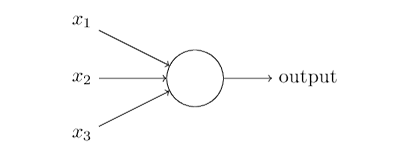
\includegraphics[width=0.5\textwidth]{Bilder/neuron.png}
    \caption{Aufbau eines künstlichen Neurons \citep{nielsen2015neural}}
    \label{fig:neuron}
\end{figure}

\subsubsection{Architektur künstlich neuronaler Netzwerke}
Ein künstliches Neuron stellt eine Funktion dar, die mehrere Eingangssignale in ein Ausgangssignal überführt \citep{nielsen2015neural}. Abbildung \ref{fig:neuron} zeigt diese Transformation anhand eines einfachen Perzeptron. Dieses ist das einfachste Modell eines künstlichen Neurons. Ein Neuron kann ein oder mehrere Eingabewerte (Inputs) $x_1, x_2, \ldots, x_n$ haben, die numerisch dargestellt sind. Sie beinhalten Informationen aus externen Datenquellen oder vorherigen Neuronen. Jedem dieser Werte ist ein Gewicht $w_i$ zugeordnet, welches die Stärke des Einflusses eines Eingangssignals auf die Ausgabe bestimmt. 

Während des Lernprozesses können diese Gewichte angepasst werden, um somit die Ausgabe und Funktionalität des Modells zu verbessern \citep{lammel2012kunstliche}. Es wird zusätzlich ein konstanter Eingabewert integriert. Dieser wird als Bias $b$ bezeichnet. Er erhöht die Flexibilität des Modells. Der Bias und die gewichteten Eingangswerte werden zu einer Gesamtsumme, der sogenannten Aktivierung, zusammengeführt. 

Die gewichtete Summe kann als Zusammenfassung aller verfügbaren Informationen verstanden und durch folgende Gleichung repräsentiert werden \citep{grum2022construction,nielsen2015neural}:
\[a = \sum_{i=1}^{n} w_i x_i + b\]
Dies ist Grundlage der Aktivierungsfunktion, die das Ausgabesignal berechnet. Die Aktivierungsfunktion transformiert die Aktivierung in einen Ausgabewert und führt häufig Nichtlinearitäten ein, wodurch komplexe Zusammenhänge modelliert werden können. Bei einem klassischen Perzeptron erfolgt eine harte Schwellwertentscheidung:
\[
\text{Ausgabe} =
\begin{cases}
1, & \text{wenn die Aktivierung } > 0 \\
0, & \text{wenn die Aktivierung } \le 0
\end{cases}
\]
Das Perzeptron kann somit als einfacher binärer Klassifikator betrachtet werden. Das Ergebnis dieser Funktion bildet dann das Ausgabesignal des Neurons. Auf diese Weise stellt ein künstliches Neuron ein neuronales Modell dar, dass nach biologischen Prinzipien funktioniert. Die Inputs repräsentieren die Dendriten und die Gewichte die Stärke der Synapsen. Die Aktivierungsfunktion entspricht dem Mechanismus, mit dem ein biologisches Neuron entscheidet, ob ein Signal weitergeleitet wird. Ausgabe des künstlichen Neurons ist das Signal, dass schließlich über das Axon an andere Neuronen übertragen wird.

Einzelne Perzeptrone können zu einem Netzwerk zusammengeschlossen werden \citep{nielsen2015neural,kinnebrock2018neuronale}. Die Ausgabe eines Neurons repräsentiert dann die Eingabe für nachfolgende Neuronen. Durch mehrere Schichten der Verarbeitung können auf diese Weise abstrakte Zusammenhänge abgebildet werden. Die Verarbeitung erfolgt schichtweise von links nach rechts. Neuronen in früheren Schichten erkennen einfache Muster und Neuronen in höhere Schichten kombinieren diese Informationen dann zu komplexeren Merkmalen. Auf diese Weise können Entscheidungsprozesse modelliert werden. Moderne Deep-Learning-Modelle verwenden häufig keine einfachen Schwellenfunktionen mehr. Stattdessen werden differenzierbare Aktivierungsfunktionen wie Sigmoid-Funktion oder Tangens-Funktion verwendet. Die Sigmoid-Funktion liefert Werte zwischen 0 und 1. Sie wird häufig für Wahrscheinlichkeitsinterpretationen verwendet. Beim hyperbolischen Tangens (tanh) sind Werte zwischen -1 und +1 um null zentriert.

\subsubsection{Training künstlicher neuronaler Netze}
Der grundlegende Lernprozess eines neuronalen Netzes wird durch die schrittweise Anpassung der Gewichte und Bias-Werte ermöglicht \citep{grum2022construction,lammel2012kunstliche}. Ziel des Trainingsprozesses ist es, die Differenz zwischen den gewünschten, gegebenen Zielwert und dem tatsächlichen Ausgabewert zu minimieren. Dieser Unterschied wird als Vorhersagefehler bezeichnet. Das Lernen erfolgt iterativ, indem der Testdatensatz mehrmals durchläuft. Es endet, wenn ein definiertes Qualitätskriterium erreicht wird oder keine wesentlichen Verbesserungen mehr auftreten. Im ersten Schritt werden die Gewichte der Verbindungen zufällig initialisiert, da noch kein Wissen über bestehende Zusammenhänge existiert. Beim Forward-Pass werden Eingabedaten ausschließlich vorwärts durch das Netz propagiert. Solche Netzwerke werden als Feedforward Neural Networks bezeichnet. Aufgrund mehrerer Schichten spricht man dann häufig von Multilayer Perzeptron (MLP). Der Fehler (Loss) beschreibt, wie stark die Vorhersage von der gewünschten Ausgabe abweicht. Häufig verwendete Fehlerfunktionen sind Mean Squared Error (MSE) oder Cross-Entropy-Loss. MSE berechnet die quadratische Abweichung zwischen Vorhersage und Zielwert. Größere Fehler werden dabei stärker bestraft, weshalb sich dieser vor allem für Regressionsprobleme eignet. Cross-Entropy-Loss wird häufig für Klassifikationsaufgaben verwendet und ermöglicht schnelles, stabiles Lernen. Es wird die Abweichung zwischen vorhergesagten Wahrscheinlichkeiten und tatsächlichen Klassen gemessen. Eine weitere Möglichkeit, wie das Modell trainiert werden kann, ist Backpropagation. Dabei wird zuerst der Fehler berechnet und anschließend von der Ausgabeschicht zur Eingabeschicht zurück propagiert. Es wird ermittelt, welchen Anteil die einzelnen Verbindungen am Gesamtfehler haben, sodass eine individuelle Anpassung der Gewichte die Ausgabe verbessert. Wie stark und in welche Richtung eine Anpassung erfolgen soll, wird durch die Gradienten angegeben. Ziel des Gradientenabstiegs ist es, die Gewichte so zu verändern, dass der Fehler minimiert wird. Die Lernrate $\alpha$ bestimmt die Gewichtsanpassung. Die Wahl der Lernrate beeinflusst maßgeblich den Trainingserfolg. Ist die Lernrate groß, führt dies zu einem schnellen Lernprozess. Jedoch besteht auf diese Weise das Risiko, das Optimum zu überschreiten. Kleinere Lernraten ermöglichen zwar ein stabileres Lernen, haben jedoch eine längere Trainingsdauer. Um Lernschwankungen zu reduzieren und lokale Minima zu überwinden, sowie die Konvergenz zu beschleunigen, kann ein Momentum herangezogen werden. Dieses verleiht dem Lernprozess eine gewisse Trägheit, indem zusätzlich auch frühere Gewichtsanpassungen berücksichtigt werden. Zusätzlich kann zwischen Batch und Online Learning unterschieden werden. Beim Batch Learning erfolgt die Gewichtsanpassung nach Verarbeitung des gesamten Trainingsdatensatzes. Dies führt zu einer stabileren Gradientenberechnung, hat jedoch einen höheren Rechenaufwand. Beim Online Learning werden die Gewichte nach jedem einzelnen Trainingsbeispiel angepasst. Dadurch wird eine schnellere Verarbeitung neuer Informationen ermöglicht. Dies ist besonders geeignet für kontinuierliche Lernprozesse, da das Verfahren robust gegenüber lokalen Minima ist. Um den Lernprozess zu verbessern ist außerdem eine Aufbereitung der Trainingsdaten hilfreich. Dies beinhaltet zum einen die Normalisierung der Daten, um die Trainingsstabilität zu verbessern und zum anderen Generalisierung. Das bedeutet, dass das Modell allgemeine Muster und Zusammenhänge erkennen kann, anstatt auf spezifische Einzelfälle zu betrachten. Das Ergebnis ist dann, eine hohe Leistung auf unbekannten Testdaten, sowie robuste Vorhersagen. Dadurch soll zudem Overfitting vermieden werden. Dies tritt auf, wenn das Netzwerk die Trainingsdaten zu genau lernt. Das bedeutet, es erlangt zwar sehr gute Ergebnisse auf den Trainingsdaten, jedoch schlechte Ergebnisse für unbekannte Daten. Gute Modelle erzielen somit auch auf neuen Daten eine hohe Vorhersagequalität. Um das zu erreichen, gilt die Generalisierungsfähigkeit als zentrales Qualitätsmerkmal neuronaler Netze.

\begin{figure}[h!]
    \centering
    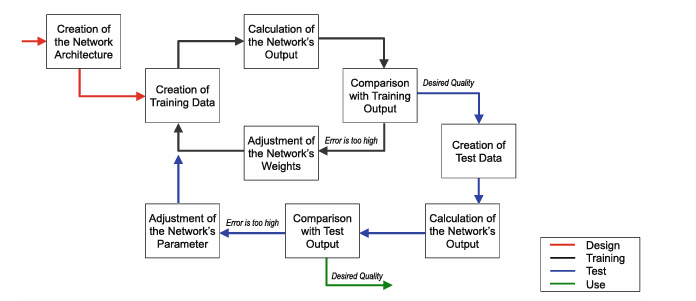
\includegraphics[width=1\textwidth]{Bilder/Training.png}
   \caption{Methodischer Ansatz zur Entwicklung neuronaler Netze \citep{lammel2012kunstliche}}
    \label{fig:training}
\end{figure}

\subsection{Promptbasierte Dialogsteuerung}
Im Kontext moderner KI-basierter Anwendungssysteme auf Basis generativer Sprachmodelle (Large Language Models) stellt das Prompt-Engineering eine zentrale Methode zur deterministischen Verhaltenssteuerung dar \citep{crocker2025softwareentwicklung}. Da autoregressive Sprachmodelle prinzipiell stochastisch operieren und Textausgaben auf Basis von Token-Wahrscheinlichkeiten generieren, dient die methodische Strukturierung der Eingabeanweisungen (Prompts) der Reduktion von Varianz und der Durchsetzung funktionaler, logischer oder tonaler Randbedingungen. In der computerlinguistischen Fachliteratur haben sich hierzu verschiedene fortgeschrittene Prompting-Techniken etabliert, die isoliert oder kombinatorisch eingesetzt werden, um die Kontrollierbarkeit und Zuverlässigkeit der Systemausgaben zu maximieren.

\subsubsection{Role Prompting}
Role Prompting basiert auf der expliziten Zuweisung einer spezifischen Systemidentität oder Rolle an das Sprachmodell innerhalb des System-Prompts \citep{zhang2023visar}. Mathematisch bewirkt diese Technik eine gezielte Konditionierung und Verengung des latenten Suchraums (Vektorraums) des Modells. Durch das Aktivieren von semantischen Clustern und Assoziationsketten, die mit der definierten Rolle korrespondieren, passt das Modell sowohl das Vokabular als auch das implizite Domänenwissen und die syntaktische Struktur der Zielausgabe an. Diese Form der Kontextualisierung verringert die Wahrscheinlichkeit von thematisch irrelevanten Ausgaben und stabilisiert die Tonalität des Dialogsystems über mehrere Interaktionsschritte hinweg.

\subsubsection{Structured Prompting}
Structured Prompting beschreibt die formale Strukturierung des Eingabetextes durch klar definierte Trennzeichen, XML/JSON-Tags oder Variablenplatzhalter \citep{hao2022structured}. Ziel dieser Technik ist es, eine eindeutige Trennung zwischen statischen Systeminstruktionen, dynamischen Kontextdaten und variablen Benutzerdatensätzen zu erzwingen. Durch die Verwendung strukturierter Masken kann ein übergeordnetes Softwaresystem externe, strukturierte Daten (z.\,B. aus Datenbanken oder algorithmischen Berechnungsebenen) zur Laufzeit dynamisch in den Prompt injizieren. Das Sprachmodell fungiert in dieser Architektur als rein ausführende generative Instanz, deren semantischer Handlungsrahmen durch die softwareseitig vorgegebenen Variablenwerte deterministisch limitiert wird.

\subsubsection{Chain-of-Thought Prompting}
Chain-of-Thought Prompting zwingt das Sprachmodell dazu, komplexe, mehrstufige Aufgabenstellungen nicht direkt zu beantworten, sondern den Transformationsprozess in eine Sequenz von logischen Zwischenschritten zu zerlegen \citep{wei2022chain}. Das Modell wird angewiesen, diesen inneren Monolog bzw. die logische Herleitung explizit zu verschriftlichen, bevor das finale Ausgabetoken generiert wird. Da LLMs Token für Token generieren, erlaubt die Erzeugung einer solchen intermediären Gedankenkette dem Modell, auf den zuvor selbst generierten logischen Zwischenschritten aufzubauen. Dies erhöht die mathematische und logische Präzision bei komplexen Schlussfolgerungsprozessen, schrittweisen Analysen oder der Einhaltung mehrstufiger, sequentieller Verhaltensregeln signifikant.

\subsubsection{Zero-Shot Prompting}
Zero-Shot Prompting beschreibt ein Verfahren, bei dem LLM eine spezifische Aufgabe ausschließlich über abstrakte Instruktionen, Regelwerke und Randbedingungen vorgegeben wird, ohne dass im Vorfeld exemplarische Eingabe-Ausgabe-Paare im Kontext hinterlegt werden \citep{brown2020language,ronanki2024requirements}. Diese Technik basiert auf der fundamentale Fähigkeit moderner, vortrainierter Transfomer-Modelle zur Generalisierung. Anstatt syntaktische Muster aus bereitgestellten Beispielen zu replizieren, dekonstruiert das Modell die abstrakte semantische Logik der Systemanweisungen und wendet sein im Pre-Training erworbenes, implizites Wissen direkt auf die neue Problemstellung an.


\section{Nutzung von KI-Chatbots im Coaching}
KI-basierte Chatbots haben in den letzten Jahren bereits vermehrt Einzug in den Coachingbereich gefunden. Sie werden zur Selbststeuerung von Personen oder Teams verwendet, um Entwicklungs- und Reflexionsprozesse zu unterstützen \citep{mai2020ai}. Coaching mit traumasensibler Ausrichtung verfolgt das Ziel, der Heilung durch Selbstregulation von Erregungszuständen und intensiven Emotionen \citep{Levine2010}. Daran anknüpfend wird eine Einordnung verschiedener Intensitäten von Belastungszuständen und psychische Belastungen herangezogen. 

Nach der NICE-Leitlinie wird zwischen milden, moderaten und schweren Störungen unterschieden \citep{kendrick2012common}. Ein milder Belastungszustand zeichnet sich durch wenig Symptome, eine begrenzte Dauer und geringe Auswirkungen auf den Alltag aus. Meist ist dies mit neu auftretenden Beschwerden oder mittelgradigen Problemen ohne Vorgeschichte verbunden. Von moderaten Belastungen spricht man, wenn eine deutliche Beeinträchtigung der Funktionalität vorliegt. Ein schwerer Belastungszustand liegt dann vor, wenn die Symptome eine erhebliche Beeinträchtigung der Funktionalität bewirken und über einen langen Zeitraum anhalten. Entsprechend ist eine intensivere Behandlung beziehungsweise Versorgung erforderlich, weshalb der Fokus dieser Arbeit auf dem Spektrum von milden bis moderaten Zuständen liegt.

\subsection{Related Work: Bisherige KI-basierte Erfolgsmodelle} \label{modell}
Im Folgenden werden zwei KI-basierte Erfolgsmodelle vorgestellt, die als Grundlage des in dieser Arbeit hergeleitete Chatbot-Modell dienen.

\subsubsection{MIND-SAFE Framework} 
Eine Referenzarchitektur für LLM-basierte Mental-Health-Chatbots ist das MIND-SAFE Framework, dessen Struktur in \ref{fig:mind} dargestellt ist. Ziel dieses Frameworks ist es, ein Dialogsystem bereitzustellen, dass therapeutisch fundiert arbeitet \citep{boit2025prompt}. Es werden ethische Standards beachtet und basiert auf einer personalisierten Struktur. Eine Kombination aus zugrundelegenden theoretischen Ansätzen und LLM Prompt Engineering führt zu einer mehrstufigen Sicherheitsarchitektur. Die erste Schicht ist der Input-Layer, der die Interaktion des Benutzers repräsentiert. Das bedeutet, der Nutzer gibt einen Text in den Chat ein, woraufhin eine Verarbeitung der Eingabe stattfindet. Es wird eine Risikoerkennung durchgeführt, um die spezifische Situation der Person zu erfassen, um vor allem gefährliche Inhalte frühzeitig zu erkennen. Die Dialog Ebene stellt den Kern des Systems dar und enthält drei zentrale Komponenten. In der User State Database wird der Zustand des Nutzers (zum Beispiel dessen Emotionen) im Zeitverlauf festgehalten, wodurch eine Personalisierung ermöglicht wird. Im zweiten Schritt erfolgt dann eine Retrieval-Argumented Generation. Das LLM greift auf eine Wissensbasis zu, die sich etablierten Therapieansätzen der kognitiven Verhaltenstherapie (CBT), Acceptance \& Commitment Therapy (ACT) oder Dialektisch-behaviorale Therapie (DBT) bedient. Dadurch wird ermöglicht, klinisch fundierte Antworten zu generieren. Der Promptengineering Layer strukturiert die therapeutische Gesprächsführung und steuert auf diese Weise Empathie, Tonalität und Interventionen. Durch das Multitier Safety System erfolgt eine mehrstufige Sicherheitsprüfung. Diese unterteilt sich in Pre-Generation Filter zur Risikoerkennung von LLM-Antworten, Post-Generation Filter zur Prüfung generierter Antworten und die Etical Guardrails, welche Regeln zur klinischen Sicherheit und zum Datenschutz beinhalten. Abschließend folgt ein kontinuierlicher Lernprozess. Dies meint eine Feedback-Schleife, wo Therapeuten und Experten die Nutzerinteraktionen prüfen und eine klinische Validierung und Verbesserung des Systems durchführen.

\begin{figure}[h!]
    \centering
    \includegraphics[width=1\textwidth]{Bilder/mind.png}
    \caption{Die Architektur des MIND-SAFE Frameworks \citep{boit2025prompt}}
    \label{fig:mind}
\end{figure}

\subsubsection{Digital Therapeutics (DTx) Komponentenmodell}
Die Grundidee des Frameworks ist ein Chatbot Modell, dass nicht nur aus einem Chatbot besteht, sondern mehrere funktionale Komponenten integriert \citep{baumel2025more}. Diese sind in \ref{fig:dtx} dargestellt. Damit soll eine höhere Wirksamkeit, Personalisierung und Skalierbarkeit therapeutischer Interventionen ermöglicht werden. Das Modell besteht aus fünf Kernkomponenten. Die Therapieeinheiten sind therapeutische Interventionen, wie Übungen oder Psychoedukation \citep{baumel2025more}. Psychoedukation verfolgt das Ziel, Klienten über eine Krankheit oder Behandlung zu informieren und damit ein Krankheitsverständnis, sowie den selbstverantwortlichen Umgang damit zu fördern \citep{bauml2018psychoedukation}.  Die KI kann an der Stelle Inhalte an Kontext oder Symptome der Klienten individuell anpassen. Die Entscheidungslogik bestimmt, wann und in welcher Reihenfolge Therapieeinheiten genutzt werden. Dies folgt dem Prinzip klassischer Entscheidungsbäume und schafft eine adaptive Anpassung an das Nutzerverhalten. Die narrative Ebene verbindet einzelnen Interventionen. Die Unterstützungsfunktion ergänzt menschliche Begleitung durch technische Hilfe. Das kann auch bedeuten, Feedback zum Verhalten zu geben oder den Nutzer zurück ins Programm zu holen. Die therapeutische Gesprächsinstanz ist die eigentlich zentrale dialogische Einheit des Systems. Die KI ermöglicht hier flexible und situationsspezifische Gespräche, Simulationen und Anpassung an Emotionen oder Zielsetzung des Prozesses. 

\begin{figure}[h!]
    \centering
    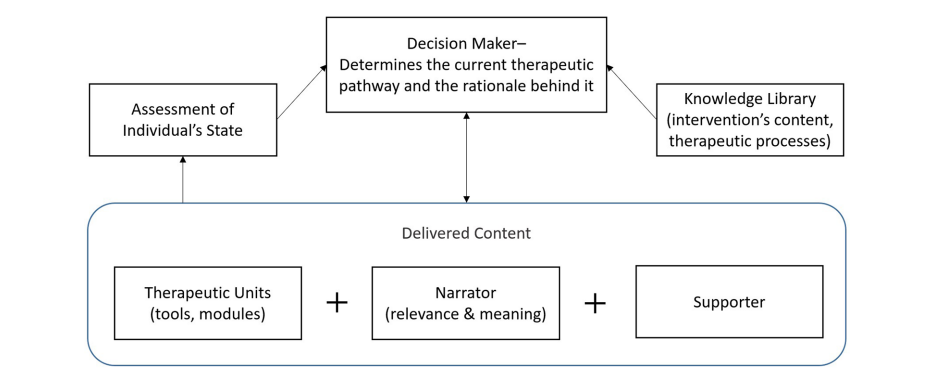
\includegraphics[width=1\textwidth]{Bilder/dtx.png}
    \caption{Die Komponenten der Digital Therapeutics \citep{baumel2025more}}
    \label{fig:dtx}
\end{figure}

\section{PSI-Theorie als psychologischer Bezugsrahmen}

Die Persönlichkeits-System-Interaktionen (PSI) Theorie nach \cite{Kuhl2000The} vereint Ansätze aus der Psychologie und Neurobiologie. Nach der PSI Theorie können kognitive und selbstregulatorische Mechanismen verändert werden. Dies wird durch die Art und Weise, wie eine Person Stimmungen und Gefühle, die sogenannten Affekte, reguliert, ermöglicht.
Die Theorie beleuchtet das menschliche Verhalten als Wechselspiel psychischer Systeme \citep{kuhl2005neue}. Es werden die vier Erkenntnissysteme Intentionsgedächnis, Intuitive Verhaltenssteuerung, Extentionsgedächnis sowie Objekterkennung unterschieden. Diese Systeme stehen in unmittelbarem Zusammenhang zueinander. Die Aktivierung der Systeme, sowie der Informationsaustausch zwischen diesen ist von den Affekten abhängig. Die Annahme der Theorie ist, dass unter Stress eine ängstliche oder traurige Stimmung vorherrscht, sodass der Mensch nicht mehr frei entscheiden kann, welches psychische System gerade aktiv ist. Bei positiver oder sicherer Stimmung hingegen besteht ein besseres Zusammenspiel der Systeme, was zur Selbstentwicklung beiträgt.


\subsection{Die vier psychischen Systeme}

\subsubsection{Intentionsgedächnis (IG)}
Das Intentionsgedächnis als analytisch sequentiell arbeitendes System ist zuständig für die Aufrechterhaltung von expliziten Absichten \citep{kuhl2005neue,kuhl2014psi}. Hier werden Ziele, Pläne und bewusste Entscheidungen gesteuert. Das IG wird besonders bei Hindernissen, Zielkonflikten oder fehlender Gelegenheit aktiv. Diese Aktivierung wird so lange aufrecht gehalten, bis eine Umsetzung des Ziels möglich ist. Dabei kommt es zur Hemmung, um vorschnelles Handeln zu vermeiden. Eine zu schwache Hemmung führt zu impulsivem Verhalten, eine zu starke kann Prokrastination, also das Aufschieben von Handlungen bewirken. Dies zeigt sich zum Beispiel, wenn man sich beim Vorhaben zu lernen ablenken lässt.

\subsubsection{Intuitive Verhaltenssteuerung (IVS)}
Die intuitive Verhaltenssteuerung ist einerseits bei der Umsetzung von Absichten und andererseits bei der Ausführung automatisierter Handlungsabläufe aktiv \citep{kuhl2014psi}. Im Gegensatz zum Intentionsgedächtnis arbeitet sie nicht primär bewusst und sequenziell, sondern verarbeitet Informationen parallel und unbewusst in Echtzeit. Dadurch ermöglicht sie ein spontanes, sensibles und situationangepasstes Verhalten, etwa in zwischenmenschlicher Kommunikation oder bei eingeübten Fertigkeiten, wie Auto fahren. Die IVS ergänzt das Intentionsgedächtnis, indem sie abstrakte Absichten in konkretes, an die jeweilige Situation angepasstes Handeln überführt.

\subsubsection{Extensionsgedächnis (EG)}
Das Extensionsgedächnis wird als (poly-)semantisches Netzwerk betrachtet, welches Aspekte wie Erfahrungen, Bedürfnisse und Werte der eigenen Person (des sogenannten Selbst) als ganzheitliches Wissen widerspiegelt \citep{kuhl2005neue,kuhl2014psi}. Dieses Wissen ist meist implizit und aus diesem Grund nicht immer vollumfänglich zugänglich. Es liefert eine Sammlung an persönlichen Lebenserfahrungen, die für die aktuelle Situation von Bedeutung sein könnten. Das EG ermöglicht die gleichzeitige
Berücksichtigung und Integration vieler Aspekte, die für komplexe Entscheidungen und gegenseitiges Verstehen von Menschen relevant sein können. Das Extensionsgedächnis und Selbst werden besonders durch persönliche Begegnungen aktiviert, bei denen gegenseitiges Verstehen eine zentrale Rolle spielt. Dies zeigt sich zum Beispiel in Partnerschaften oder auch der Verbindung zwischen Coach und Klient. Das EG kann Informationen und Gefühle simultan verarbeiten und integrieren, im Gegensatz zum analytisch-sequenziellen Denken des Intentionsgedächtnisses. Es ist für die Integration komplexer Erfahrungen relevant und ermöglicht insbesondere durch die Verarbeitung negativer Erlebnisse Selbstentwicklung und Lernsprünge. Dadurch zeigt sich wie bedeutend der Zugang des EG zur Selbstwahrnehmung für die Regulation von Gefühlen und damit auch die Verarbeitung negativer Erfahrungen ist.


\subsubsection{Objekterkennungssystem (OES)}
Das Objekterkennungssystem ermöglicht die bewusste Wahrnehmung einzelner, aus dem Gesamtkontext herausgelöster Aspekte und richtet die Aufmerksamkeit besonders auf Neuartiges, Fehler oder potenzielle Gefahren \citep{kuhl2005neue,kuhl2014psi}. Negative Stimmungen verstärken dabei den Fokus auf Unstimmigkeiten und Details, wie zum Beispiel das Versprechen während einer Präsentation. Das OES nimmt Einzelaspekte isoliert wahr, indem es sie aus dem Gesamtzusammenhang herauslöst. Das Extensionsgedächtnis integriert diese wieder in größere Zusammenhänge. Das Zusammenspiel beider Systeme ist wichtig für Lernen, Selbstentwicklung und situationsangemessenes Denken. Dabei hilft das OES beim Erkennen von Fehlern und Gefahren, das EG beim ganzheitlichen Verstehen und Einordnen von Erfahrungen.

\subsection{Modulationsannahmen der PSI-Theorie}
Die PSI-Theorie geht davon aus, dass positive und negative Affekte (Stimmungen und Gefühle) die Aktivierung und das Zusammenspiel der psychischen Systeme steuern \citep{kuhl2014psi}. Affekte beeinflussen die Aktivierung und Interaktionen der Systeme.  Gleichzeitig wirken die psychischen Systeme selbst wieder auf Affekte zurück. \cite{kuhl2014psi} beschreibt zwei zentrale Modulationsannahmen, die erklären, wie Affekte das Zusammenspiel der psychischen Systeme beeinflussen: 
\begin{enumerate}
  \renewcommand{\labelenumi}{(\arabic{enumi})}
  \item Willensbahnung: Die Umsetzung von Absichten durch die Zusammenarbeit von Intentionsgedächtnis (IG) und Intuitiver Verhaltenssteuerung (IVS)
  \item Selbstentwicklung durch Affektregulation: Selbstentwicklung durch die Interaktion von Objekterkennungssystem (OES) und Extensionsgedächtnis (EG)
\end{enumerate}

\subsubsection{Erste Modulationsannahme: Willensbahnung}
Die erste Modulationsannahme ist die Willensbahnung, die durch die Entstehung eines positiven Affekts und damit einem aktiven Intentionsgedächnisses entsteht \citep{Kuhl2000The}. Ein positiver Affekt erleichtert das Umsetzen von Intentionen, weil es eine höhere Bereitschaft zur Umsetzung gewährleistet. 

Das IG speichert Ziele und Absichten \citep{kuhl2005neue, kuhl2014psi}. Es wird besonders bei schwierigen oder unangenehmen Aufgaben aktiv und hält die Intention aufrecht. Herausforderungen reduzieren jedoch häufig den positiven Affekt, was dazu führen kann, dass die Umsetzung blockiert wird. Positive Affekte haben in diesem Zusammenhang eine entscheidende Rolle, weil sie das IVS aktivieren. Dadurch werden Hemmungen reduziert und flüssiges, spontanes Handeln ermöglicht. Statt die Absicht nur zu planen, kann eine tatsächliche Handlung entstehen. Positive Affekte, die dies ermöglichen, sind beispielsweise Motivation, Zuversicht, Ermutigung oder die Vorstellung eines erfolgreichen Ergebnisses.

\cite{kuhl2005neue} beschreibt die Fähigkeit der Frustrationstoleranz, wobei schwierige Absichten aufrechterhalten werden können, wenn negative Gefühle kurzfristig ausgehalten werden. Zur tatsächlichen Umsetzung von Absichten ist die Pendeltechnik geeignet. Diese basiert auf einem Wechsel von 1. der positiven Vorstellung des Zieles, 2. der bewussten Auseinandersetzung mit Schwierigkeiten und 3. der erneuten Aktivierung positiver Gefühle. Grundlage dessen ist ein flexibles Wechseln zwischen beiden Zustände.


\subsubsection{Zweite Modulationsannahme: Selbstentwicklung durch Affektregulation}
Die zweite Modulationsannahme beschreibt das Zusammenspiel von Objekterkennungssystem (OES) und Extensionsgedächtnis (EG) \citep{kuhl2005neue, kuhl2014psi}. Dabei wird das OES durch einen negativen Affekt aktiviert. Die Aufmerksamkeit richtet sich stärker auf Fehler, Unstimmigkeiten oder einzelne negative Aspekte, was dazu führt, dass der ganzheitliche Überblick verloren geht. Der Zugang zum Extensionsgedächtnis (EG) wird gehemmt, was zur Folge hat, dass negatives Denken die Wahrnehmung verengt und positive Erfahrungen oder alternative Sichtweisen weniger wahrgenommen werden. Auch der Zugang zu den eigenen Werten, Bedürfnissen oder Erfahrungen kann erschwert werden. Wenn der negative Affekt wieder reguliert wird, ist der Zugang zum EG erneut möglich, was Selbstwahrnehmung und die Integration von Erfahrungen fördert. Auf diese Weise ist Selbstreflexion, die Verarbeitung von Emotionen und damit eine Entwicklung möglich. Bei langanhaltenden negativen Affekten kann es passieren, dass fremde Ziele als eigene wahrgenommen werden und der Zugang zu den eigenen Bedürfnissen schwerfällt. Dies wird als Selbstfiltration bezeichnet und zeigt sich zum Beispiel, wenn eine Person die Erwartungen anderer übernimmt, ohne zu merken, dass diese nicht den eigenen Werten entspricht.

\begin{figure}[h!]
    \centering
    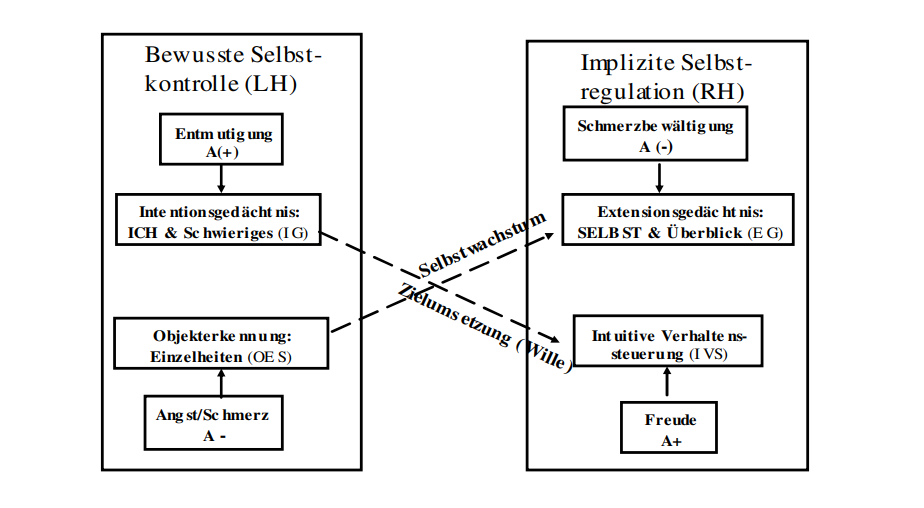
\includegraphics[width=1\textwidth]{Bilder/Modulationsannahmen.png}
    \caption{Schematische Darstellung der PSI-Theorie nach \cite{kuhl2005neue}}
    \label{fig:ma_kuhl}
\end{figure}

\subsubsection{Emotionale Steuerung von Verhalten}
Affektregulation wird als Grundlage von Willenskraft und Selbstentwicklung betrachtet und stellt somit eine zentrale Voraussetzung für die Selbststeuerung dar \citep{kuhl2005neue}. Das Zusammenspiel der einzelnen Systeme, Affekte und Modulationsannahmen sind in Abbildung \ref{fig:ma_kuhl} dargestellt. Selbstmotivierung entsteht durch die Regulation positiver Affekte und unterstützt somit die Umsetzung von Zielen. Selbstberuhigung ermöglicht die Verarbeitung belastender Erfahrungen, durch die Regulation von negativen Affekten. Der flexible Wechsel zwischen positiven und negativen Affekten wird als emotionale Dialektik bezeichnet. Weder dauerhaft positive noch dauerhaft negative Stimmung ist förderlich. Grundlage der Persönlichkeitsentwicklung ist die Fähigkeit, bewusster Selbstkontrolle und Gefühle situationsangemessen zu regulieren. Auf diese Weise fördern positive Affekte die Handlungsumsetzung (Willensbahnung), während negative Affekte helfen, Fehler und Probleme wahrzunehmen. Die anschließende Regulation negativer Gefühle ermöglicht Selbstreflexion und Lernen. 

Die Fähigkeit, Affekte eigenständig regulieren zu können, wird als Selbstkompetenz bezeichnet \citep{kuhl2014psi}. Dieser Lernprozess kann nur dann erfolgreich integriert werden, wenn die Beruhigung der Gefühle aus sich heraus bewältigt werden können, das heißt, wenn das „selbst“ in diesem Augenblick aktiv war. Eine positive Reaktion kann vor allem dann verknüpft werden, wenn Verständnis durch den Interaktionspartner gegeben ist. In der PSI-Theorie wird diese Verknüpfung der zwei Systeme, der affektiven Reaktion und des Selbst als Selbstkonditionierung bezeichnet.


\subsection{Bedeutung für Coachingprozesse} \label{prozess}
Die PSI-Theorie bietet eine gute Möglichkeit für Coachingprozesse, um Interventionen und Methoden abzuleiten \citep{kuhl2005neue}. Aus den Modulationsannahmen und damit der Integration der vier Systeme ergibt sich eine wichtige Implikation für Coachingprozesse. Demnach funktioniert Persönlichkeitsentwicklung umso besser, je besser die vier psychischen Systeme zusammenarbeiten. Selbstregulationsfähigkeiten entwickeln sich vor allem in Beziehungen. Gegenseitiges Verstehen gilt als zentrale Voraussetzung für Entwicklung. Auch emotionale Dialektik spielt im Coachingkontext eine elementare Rolle. Der Coach kann dem Klienten dabei helfen, Emotionen richtig Einzuordnen und sich nicht in emotionalen Zuständen zu verlieren, sondern Gefühle zu verarbeiten und für Motivation, sowie die Umsetzung einer Handlung zu nutzen. Zentrale Qualitäten vom Coaching sind im Kontext der PSI-Theorie, den Zugang zum Selbstsystem zu fördern, Selbstmotivierung zu stärken, Selbstberuhigung zu unterstützen, selbstkonguente Ziele zu entwickeln, emotionale Selbstregulation zu fördern und damit eine langfristige Selbststeuerung und Persönlichkeitsentwicklung zu ermöglichen. Coaching wirkt nicht primär durch Ratschläge, sondern durch eine zwischenmenschliche Beziehung.

\subsubsection{Schwerpunkt Selbstmotivierung (Erste Modulationsannahme)}
Die Pendeltechnik beschreibt den Wechsel zwischen positiven und negativen Affekten \citep{kuhl2005neue}. Es kann ein Perspektivwechsel zwischen Problembezogenheit und Ressourcenorientiertierung ermöglicht werden. Das Ziel besteht darin, nicht dauerhaft in einem negativen emotionalen Zustand zu verbleiben. Negative Gefühle werden also nicht einfach vermeiden oder unterdrückt, sondern die Fähigkeit zwischen emotionalen Zuständen flexibel wechseln können ermöglicht. Dadurch können belastende Erfahrungen wahrgenommen und verarbeitet werden. Gleichzeitig können positive, ressourcenorientierte Zustände zugänglich bleiben und emotionale Verarbeitung kann mit Motivation und Handlungsfähigkeit verbunden werden. Wenn der Fokus nicht ausschließlich auf Problemen oder Defiziten liegt, kann eine gezielte Aktivierung bereits vorhandener Ressourcen zu einem persönlichen Wachstum beitragen. Dadurch wird Zuversicht gefördert, Selbstwirksamkeit gestärkt, der Zugang zu positiven Erfahrungen ermöglicht und die Perspektive auf eigene Handlungsmöglichkeiten erweitert. Auf diese Weise wird wieder Verbindung zum EG, Selbstzugang, Integration und zur Handlungsaktivierung geschaffen. 

Die PSI-Theorie erklärt, dass Motivation und Zuversicht die Aufrechterhaltung von Absichten unterstützen können und das Vorstellen eines erfolgreichen Ergebnisses relevante psychische Systeme aktivieren können \citep{kuhl2005neue,kuhl2014psi}.

\subsubsection{Schwerpunkt Selbstberuhigung (Zweite Modulationsannahme)}
Unterstützung bei belastenden Erfahrungen und negativen Emotionen kann die Selbstberuhigung erleichtern \citep{kuhl2005neue, kuhl2014psi}. Der Coach kann den Klienten aus negativen Gedanken und Grübeln herausholen und stattdessen einen ganzheitlichen Blick auf die Situation liefern. Dies fördert die Integration neuer Erfahrungen in das Selbstsystem. Die Aktivierung des EG erfolgt besonders dann, wenn Menschen sich verstanden, gesehen und akzeptiert fühlen. Eine vertrauensvolle Beziehung, wie sie zwischen Coach und Klient gegeben sein sollte, kann den Zugang zu eigenen Ressourcen und Erfahrungen erleichtern und somit einen Rahmen schaffen, in dem diese eigenen Fähigkeiten gestärkt werden. 
Die Förderung der emotionalen und körperbezogenen Selbstwahrnehmung (des EG) kann an dieser Stelle eine Unterstützung darstellen \citep{storch2007ressourcenorientiertes}.

Ein Coach kann zum Beispiel bei der Regulation von Affekten eine Hilfe sein \citep{kuhl2014psi}. Die Verarbeitung negativer Erfahrungen gelingt nachhaltig vor allem dann, wenn sie emotional in das Selbstsystem integriert werden, statt lediglich kognitiv analysiert zu werden. Reines Reflektieren und argumentative Einordnung reichen dafür oft nicht aus, selbst wenn sie inhaltlich stimmig oder tröstlich erscheinen. 

Wiederholte positive Erfahrungen wie Trost, Ermutigung oder Verständnis fördern die Entwicklung der Selbstregulation, sodass langfristig positive emotionale Zustände selbstständig erzeugt werden können \citep{storch2007ressourcenorientiertes}. Wenn der Klient lernt, diese Funktionen schrittweise selbst zu übernehmen, kann emotionale Selbstständigkeit und Beziehungsfähigkeit gefördert werden. Unterstützung bei der Umsetzung schwieriger Ziele kann zur Selbstmotivierung beigetragen. Indem der Coach Interventionen zur Aktivierung persönlicher Ressourcen und Erfolgserfahrungen anleitet, kann der Klient einen besseren Zugang zum EG erlangen. Auf diese Weise kann die Entwicklung von Zuversicht gefördert werden. Durch die Regulation von Affekten kann eine Beruhigung belastender Gefühle zur Wiederherstellung eines Zustands führen, in dem weitere Verarbeitung möglich wird. Langfristig soll der Nutzer zunehmend zur Selbstberuhigung befähigt werden. Mögliche Schritte in diesem Kontext sind die Gefühle wahrnehmen und benennen und die Situation verlangsamen. Indem die Aufmerksamkeit auf regulierende und stabilisierende Aspekte gelenkt wird, Ressourcen aktiviert und Selbstberuhigung unterstützt wird. Interventionen sollen nicht ausschließlich auf kognitive Reflexion ausgerichtet sein. Auch die Wahrnehmung von Emotionen und Körperempfindungen spielt eine wichtige Rolle. Das Ziel besteht darin die Verbindung zwischen Körper, Emotion und persönlicher Bedeutung herzustellen. 
Durch die Reflexion von Werten und Bedürfnissen kann eine bewusste Unterscheidung zwischen den eigenen und fremden Erwartungen begünstigt werden. Ein Coachingziel kann somit die Vermeidung von Selbstinfiltration und Fremdbestimmung sein und damit auf die Entwicklung authentischer und persönlich passender Ziele ausgerichtet sein. Belastende oder neue Erfahrungen sollen nicht ausschließlich vermieden werden. Das Ziel ist eine Verarbeitung und Integration in den persönlichen Erfahrungskontext. Dadurch wird die Möglichkeit, aus Erfahrungen zu lernen und neue Handlungsmöglichkeiten zu entwickeln gespiegelt. Der Klient realisiert, wie er positiv mit Situationen umgeht und für sich selbst mehr Kapazität und Handlungsmöglichkeiten entwicklet. 


\subsection{Die sieben Systemebenen der PSI-Theorie}
Die PSI-Theorie betrachtet sieben Systemebenen, die menschliches Verhalten, bezüglich Umsetzung und Meidung der Motivation sowie entsprechende Affekte und Emotionen beschrieben \citep{kuhl2004systemdiagnostik, kuhl2014psi}. Im Kontext der Systemdiagnostik kann die Komplexität der Persönlichkeit im Gegensatz zu vielen klassischen Diagnostikansätzen detaillierter abgebildet werden. Klassische Persönlichkeitstests erfassen meist ausschließlich Persönlichkeitsmerkmale, sogenannte Erstreaktionen. Nach der Entwicklungsorientierten Osnabrücker Systemdiagnostik (EOS) wird außerdem betrachtet, wie eine Person mit Gedanken, Gefühlen und Problemen umgeht. Diese Selbstregulationsprozesse werden als Zweitreaktion bezeichnet. Anstatt Konstrukte wie „Selbstwirksamkeit“ oder „Persönlichkeit“ zu messen, betrachtet EOS über 100 Mikrofunktionskomponenten der Persönlichkeit, um konkrete Stärken und Entwicklungsfelder zu identifizieren. Coaching ist vor allem darauf ausgerichtet, wie eine Person Emotionen reguliert, mit Stress umgeht oder ihre Ressourcen aktiviert. Nach der EOS-Diagnostik wird ein zentraler Entwicklungshebel identifiziert, wodurch sich viele Verhaltensweisen erklären lassen. Coaching fokussiert sich demnach auf individuelle statt standardisierte Interventionen sowie emotionale Selbstregulation. Negative Emotionen werden nicht als Problem betrachtet, sondern als wichtige Information über Konflikte und Bedürfnisse. Diese Betrachtung steht in direktem Zusammenhang zur zweiten Modulationsannahme der PSI-Theorie.

Dieser Ansatz ist von besonderer Relevanz für Coachings, vor allem auch im traumasensiblen Arbeiten. Traumaheilung entsteht durch die Fähigkeit, Erregungszustände selbst zu regulieren und intensive Emotionen halten und verarbeiten zu können \citep{Levine2010}. EOS und Traumaarbeit fokussieren eine Prozess- statt Defizitorientierung, sowie die Ausrichtung auf selbstregulatorische Prozesse.

Darauf basierend werden sieben Quellen der menschlichen Motivation abgeleitet, die einen Leitfaden für Coachings liefern, um unter Betrachtung der Erst- und Zweitreaktion erfolgreiche Interventionen und Konzepte abzuleiten \citep{kuhl2004systemdiagnostik, kuhl2014psi}. 

\subparagraph{1) Automatisches Verhalten und Erkennen}
Diese Ebene umfasst gelernte Routinen und automatische Handlungen. Verhalten oder eine Reaktion wird automatisch durch einen entstehenden Reiz ausgelöst und braucht somit keine bewusste Steuerung. Wenn keine förderlichen Gewohnheiten existieren, bestehen Schwierigkeiten beim Aufbringen von Motivation.

\subparagraph{2) Temperament}
Temperament stellt die grundsätzliche Erregbarkeit und Aktivierung einer Person dar. Das bedeutet, wie stark wird auf einen Reiz reagiert und wie ist die generelle Handlungsenergie. Eine zu geringe Aktivierung kann zur Antriebslosigkeit führen, während eine besonders hohe Aktivierung zu Unruhe und Impulsivität führt.

\subparagraph{3) Affekte und Anreize}
Die dritte Ebene beschreibt die emotionale Bewertung von Erfahrungen. Auf der einen Seite stehen positive Affekte wie Freude oder Belohnung und demgegenüber negative Affekte, wie Angst, Ärger oder Stress. Motivation entsteht demnach durch eine Verknüpfung von Objekten mit Emotionen. Fehlende Motivation zum Lernen besteht zum Beispiel, wenn das Lernen negativ assoziiert ist.

\subparagraph{4) Stressbewältigung}
Bei der Stressbewältigung geht es darum, ob unter Stress eine höhere Steuerung erhalten bleibt. Progression bedeutet, dass eigene Ziele und Selbststeuerung aktiv bleiben. Regression andererseits meint einen Rückfall in impulsives Verhalte, Affekte oder Gewohnheiten. Unter Stress kann somit das Reaktionsvermögen verloren gehen.

\subparagraph{5) Motive: Kraftquellen}
Motive sind unbewusste Bedürfnisse wie beispielsweise Anerkennung, Macht, Beziehung oder Autonomie. Sie wirken oft implizit und steuern eine langfristige Zielausrichtung. Werden diese Ziele und Bedürfnisse angesprochen, kann das intrinsische Motivation, wenn auch unbewusst, erhöhen.

\subparagraph{6) Denken und Fühlen}
Als kognitive Ebene werden bewusste Gedanken, konkrete Ziele und Bedeutungsstrukturen betrachtet. Das eigene Selbstbild und Sinnzuschreibungen spielen in diesem Kontext eine Rolle zur Motivation, in dem sie Orientierung und Identifikation liefern.

\subparagraph{7) Selbststeuerung}
Die Selbststeuerung wird als höchste Ebene verstanden. Sie koordiniert das Zusammenwirken der einzelnen Systeme Selbstkontrolle, Selbstregulation, Selbstmotivierung und das Lernen aus Erfahrungen. \citep{ritz2008personlichkeitsorientierte, kuhlsieben}


\section{Systematische Literaturübersicht}
Die Vorgehensweise der Literaturrecherche folgt dem systematischen Aufbau nach \cite{webster2002analyzing}. Für die Stichwortsuche wurden die Literaturdatenbanken Google Scholar, ScienceDirect, Ieeeexplore und Scopus herangezogen. Faktoren wie Zitationen des gefundenen Artikels und 
Reputation der Autoren wurden verwendet, um einzuschätzen, ob es sich um eine hochwertige wissenschaftliche Quelle handelt. Es wurden Suchwörter wie \glqq Chatbot and Coaching\grqq{} or \glqq PSI and Coaching\grqq{} or \glqq LLM and Coaching\grqq{} eingegeben, um passende Literatur zu finden. Im zweiten Schritt folgte eine Rückwärtssuche, in der anhand der Referenzen der gefundenen Artikel aus dem ersten Schritt weitere relevante Artikel überprüft und in die Suche miteinbezogen wurden. 
Mit der daraus resultierenden Sammlung an 
Artikeln und Büchern wurde im letzten Schritt eine Vorwärtssuche durchgeführt und es entstand ein Pool an 
relevanten Artikeln. Zuletzt folgte eine intensive Auseinandersetzung mit iterativer Aussortierung der 
nicht-relevanten Artikel und Beiträge, die thematisch nicht zur Forschungsfrage passen.

\subsection{Forschungslücke}

Obwohl sich KI-gestützte Chatbots im Coaching- und therapeutischen Sektor zunehmend als digitale Selbstcoaching-Tools etablieren \citep{mai2023chatbots} und erste klinisch fundierte Referenzarchitekturen wie das MIND-SAFE Framework existieren \citep{boit2025prompt}, offenbart die systematische Literaturanalyse Forschungslücken an der Schnittstelle zwischen Wirtschaftsinformatik, dialogischer KI und psychologischer Systemtheorie.

Eine Forschungslücke ergibt sich aus der fehlenden informationstechnischen Modellierung der PSI-Theorie. Bestehende Mental-Health-Anwendungen stützen sich vorwiegend auf die algorithmische Abbildung klassischer, strukturell linearer Ansätze wie der kognitiven Verhaltenstherapie (CBT) oder der Dialektisch-behavioralen Therapie (DBT) \citep{boit2025prompt}. Es fehlt jedoch an einer operationalisierten Entscheidungs- und Dialogsteuerungslogik, die auf ganzheitlichen, neurobiologisch fundierten Persönlichkeits-System-Interaktionen (PSI) basiert \citep{Kuhl2000The}. Die computerlinguistische Modellierung des dynamischen Zusammenspiels zwischen den vier Makrosystemen (IG, IVS, EG, OES) und deren affektiver Modulation ist in der aktuellen Literatur nicht vorhanden.
    
Ein zweiter Kernpunkt stellen aktuelle Forschungsansätze im Bereich der Personalisierung des LLM dar. Diese fokussieren sich primär darauf, Interaktionen und Inhalte an die individuellen Nutzerpräferenzen anzupassen \citep{Tan2024}. Im traumasensiblen Coaching birgt diese rein reaktive Anpassung jedoch das Risiko, dass das generative Sprachmodell nicht-entwicklungsfördernden Verhaltens- und Denkmuster des Klienten adaptiert, spiegelt und somit unbewusst verfestigt \citep{Xiao2025Humanizing}. Es existiert eine Forschungslücke hinsichtlich der Frage, wie dialogische KI durch proaktive, theoriegeleitete Impulse so gestaltet werden kann, dass sie diese traumabedingten Schutzstrategien sichtbar macht, aktiv hinterfragt und transformiert, anstatt sie lediglich stochastisch zu reproduzieren.

Des Weiteren wurde ein Mangel an deterministischen Design- und Interaktionsmerkmalen für traumasensible LLMs herausgestellt. Die Arbeit knüpft an dieser Stelle an und zeigt eine präzise funktionale Ausgestaltung von Prompts, die sowohl diagnostisch als auch affektregulierend wirken \citep{kuhl2004systemdiagnostik, Levine2010}. Bisher stellt dies im Kontext von Personen mit leichten bis moderaten psychischen Belastungen eine Lücke der Forschung dar.

Während die technische Machbarkeit von dialogischer KI weit fortgeschritten ist, fehlt es an der theoretisch-konzeptionellen Ausarbeitung, die psychologische Wirkmechanismen der Affektregulation und Selbststeuerung in eine deterministische Systemarchitektur überführen. Diese Lücke wird durch das in dieser Arbeit entwickelte PSI-basierte Coaching-Modell adressiert.

    \clearpage{\pagestyle{empty}\cleardoublepage}
    \input{./Kapitel/ergebnisse}
    \clearpage{\pagestyle{empty}\cleardoublepage}
    \chapter{Design}

In Kapitel \ref{chap:2} wurde die PSI-Theorie detailliert beschrieben. Sie erklärt verschiedene Funktionszustände eines Menschen, und liefert damit eine fundierte Grundlage für die Entwicklung eines KI-basierten Chatbots, der im Coaching Bereich einsetzbar sein soll. Im Folgenden wird ein Modell konzeptionell beschreiben, dass diese Kriterien erfüllt und somit als Werkzeug für Coachings mit traumasensibler Ausrichtung dienen soll. Es wird eine PSI-basierte Dialogsteuerungslogik für ein traumasensibles Coaching-System entwickelt und evaluiert. Ziel des Modells ist, es dem hohen Bedarf an Coaches und Therapeuten entgegenzuwirken, indem zu persönlichen Denk- und Entscheidungsmustern weitere Optionen und Handlungsmöglichkeiten offenbart werden. Menschen agieren aufgrund ihrer Prägung, Erziehung, Sozialisierung oder Traumatisierung oft nach ihnen bekannten Strategien. Dadurch besteht das Problem, oft in persönlichen Verhaltensmustern festzuhängen \citep{re1989compulsion}. Das KI-Modell soll an dieser Stelle ansetzen und eine Unterstützung gewährleisten. Der Fokus des Modells liegt auf leichten bis moderaten Belastungen. Für Klienten, die sich in einem solchen Zustand befinden, soll es als ein Tool zur Selbstregulierung und -entwicklung dienen. Für Personen mit schweren Belastungszuständen ist das Modell hingegen nicht geeignet. Es wird davon ausgegangen, dass in solchen Fällen eine professionelle Hilfe, beispielsweise einee therapeutische oder klinische Behandlung, herangezogen werden sollte.

Fokus des entwickelten Modells ist es, selbstregulatorische Prozesse zu unterstützen. Damit sollen Erregungszustände und intensive Emotionen verarbeitet und Traumaheilung gefördert werden. Die Grundidee eines reflektierenden KI-Systems ist, dass es nicht nur auf Aussagen reagiert, sondern zusätzlich individuelle Muster des Nutzers erkennen und im Gesprächsverlauf aufgreifen kann. Es soll keine klinische Diagnose oder Bewertung der Strategien vorgenommen werden, sondern durch ein sichtbar machen die persönliche Selbstreflexion gefördert werden. Spiegelung individueller Muster meint, wiederkehrende Verhaltensmuster zu erkennen und diese aktiv infrage zu stellen. Das KI-System soll somit zur Reflexion und potenziellen Veränderung beitragen, indem dem Nutzer zusätzliche Perspektiven aufgezeigt werden \citep{Xiao2025Humanizing}. Persönlichkeitsentwicklung lässt sich durch das Zusammenspiel der vier psychischen Systeme erklären. Selbstregulationsfähigkeiten entwickeln sich insbesondere in Beziehungen und gegenseitiges Verstehen gilt als wichtige Voraussetzung für Entwicklung \citep{kuhl2005neue,kuhl2014psi}. Für die Übertragung auf die Mensch-Maschine-Interaktion bedeutet das, der Nutzer soll sich verstanden fühlen, individuelle Perspektiven aufgegriffen, sowie Erfahrungen und Bedürfnisse berücksichtigt werden. Interaktion sollen nicht ausschließlich auf eine schnelle Problemlösung ausgerichtet sein, sondern stattdessen ein Raum für Reflexion und Selbstwahrnehmung geschaffen werden.

\section{Integriertes Framework}
Die strukturelle Ausgangsbasis des PSI-Coaching Frameworks bilden das MIND-SAFE und DTx-Komponentenmodell, die in Kapitel~\ref{modell} beschrieben wurden. Die PSI-Theorie liefert zusätzlich eine spezifische Steuerungs- und Adaptionslogik, durch die die bestehenden Komponenten erweitert werden. Im Folgenden wird das Modell ausführlich erklärt. \\
Grundlegend besteht das Modell aus 7 aufeinanderfolgenden Ebenen. Die erste Ebene spiegelt die Nutzereingabe wider. Hier formuliert der Nutzer des Systems sein Anliegen. Im zweiten Schritt folgt eine Sicherheitsprüfung basierend auf der Logik des MIND-SAFE Frameworks \citep{boit2025prompt}. Das bedeutet konkret, dass das System prüft, ob möglicherweise eine akute Gefährdung, wie beispielsweise Suizidalität vorliegt. In diesem Fall würde eine Eskalation erkannt werden und der Nutzer an eine professionelle Hilfestelle weitergeleitet werden. Ist das Ergebnis des Sicherheitschecks nicht kritisch, kommt die nächste Ebene, in der eine PSI-Zustandsanalyse durchgeführt wird. Dieser Schritt ist ein spezifisch für das Modell entwickelte Bestandteil. Dabei werden die Eingaben und Kontextinformationen analysiert. Die Bestimmung des funktionalen PSI-Zustandes erfolgt auf Basis mehrerer Kriterien. Diese orientieren sich an den 7 Systemebenen der Entwicklungsorientierten Osnabrücker Systemdiagnostik \citep{kuhl2004systemdiagnostik}. Das Ergebnis stellt dann eine PSI-Zustandshypothese dar (z.B. OES-dominant). Darauf folgt dann die PSI-Entscheidungsebene, die PSI-basierte Ziele definiert und untersucht, welches für die gegebene Situation passend ist. Auf dieser Grundlage wird geprüft, wie ein möglicher Wechsel der Systeme durch Steuerungsmechanismen möglich ist. In der nächsten Ebene wird dann eine passende Intervention ausgewählt. Dem liegt die Frage zugrunde, welche PSI-Funktion gefördert werden soll. Die Auswahl erfolgt nach dem DTx-Modell. Interventionsziel und -typ ergeben sich aus der Therapie- und Interventionseinheit, der Entscheidungslogik, narrativen Ebene, Unterstützungsfunktion und der therapeutischen Gesprächsinstanz. Abschließend erfolgt die Generierung der Antwort an den Nutzer. Im Gesamten basiert dieser Schritt auf dem Nutzerzustand, PSI-Ziel, der gewählten Intervention, Coaching-Prinzipien und Sicherheitsvorgaben. Am Ende und damit in der letzten Ebene erfolgt ein Update des Zustandes und Feedback. Durch die Nutzerreaktion und neuer Kontextinformationen wird der PSI-Zustand aktualisiert und damit eine Grundlage für die nächste Interaktion geschaffen.
Allildung \ref{fig:psi-chatbot-ablauf} stellt den Ablauf des entwickelten PSI-basierten Chatbots dar. Die einzellnen Schritte und Ebenen werden im Folgenden detailliert beschrieben.

\begin{figure}[htbp]
\centering
\resizebox{0.95\textwidth}{!}{%
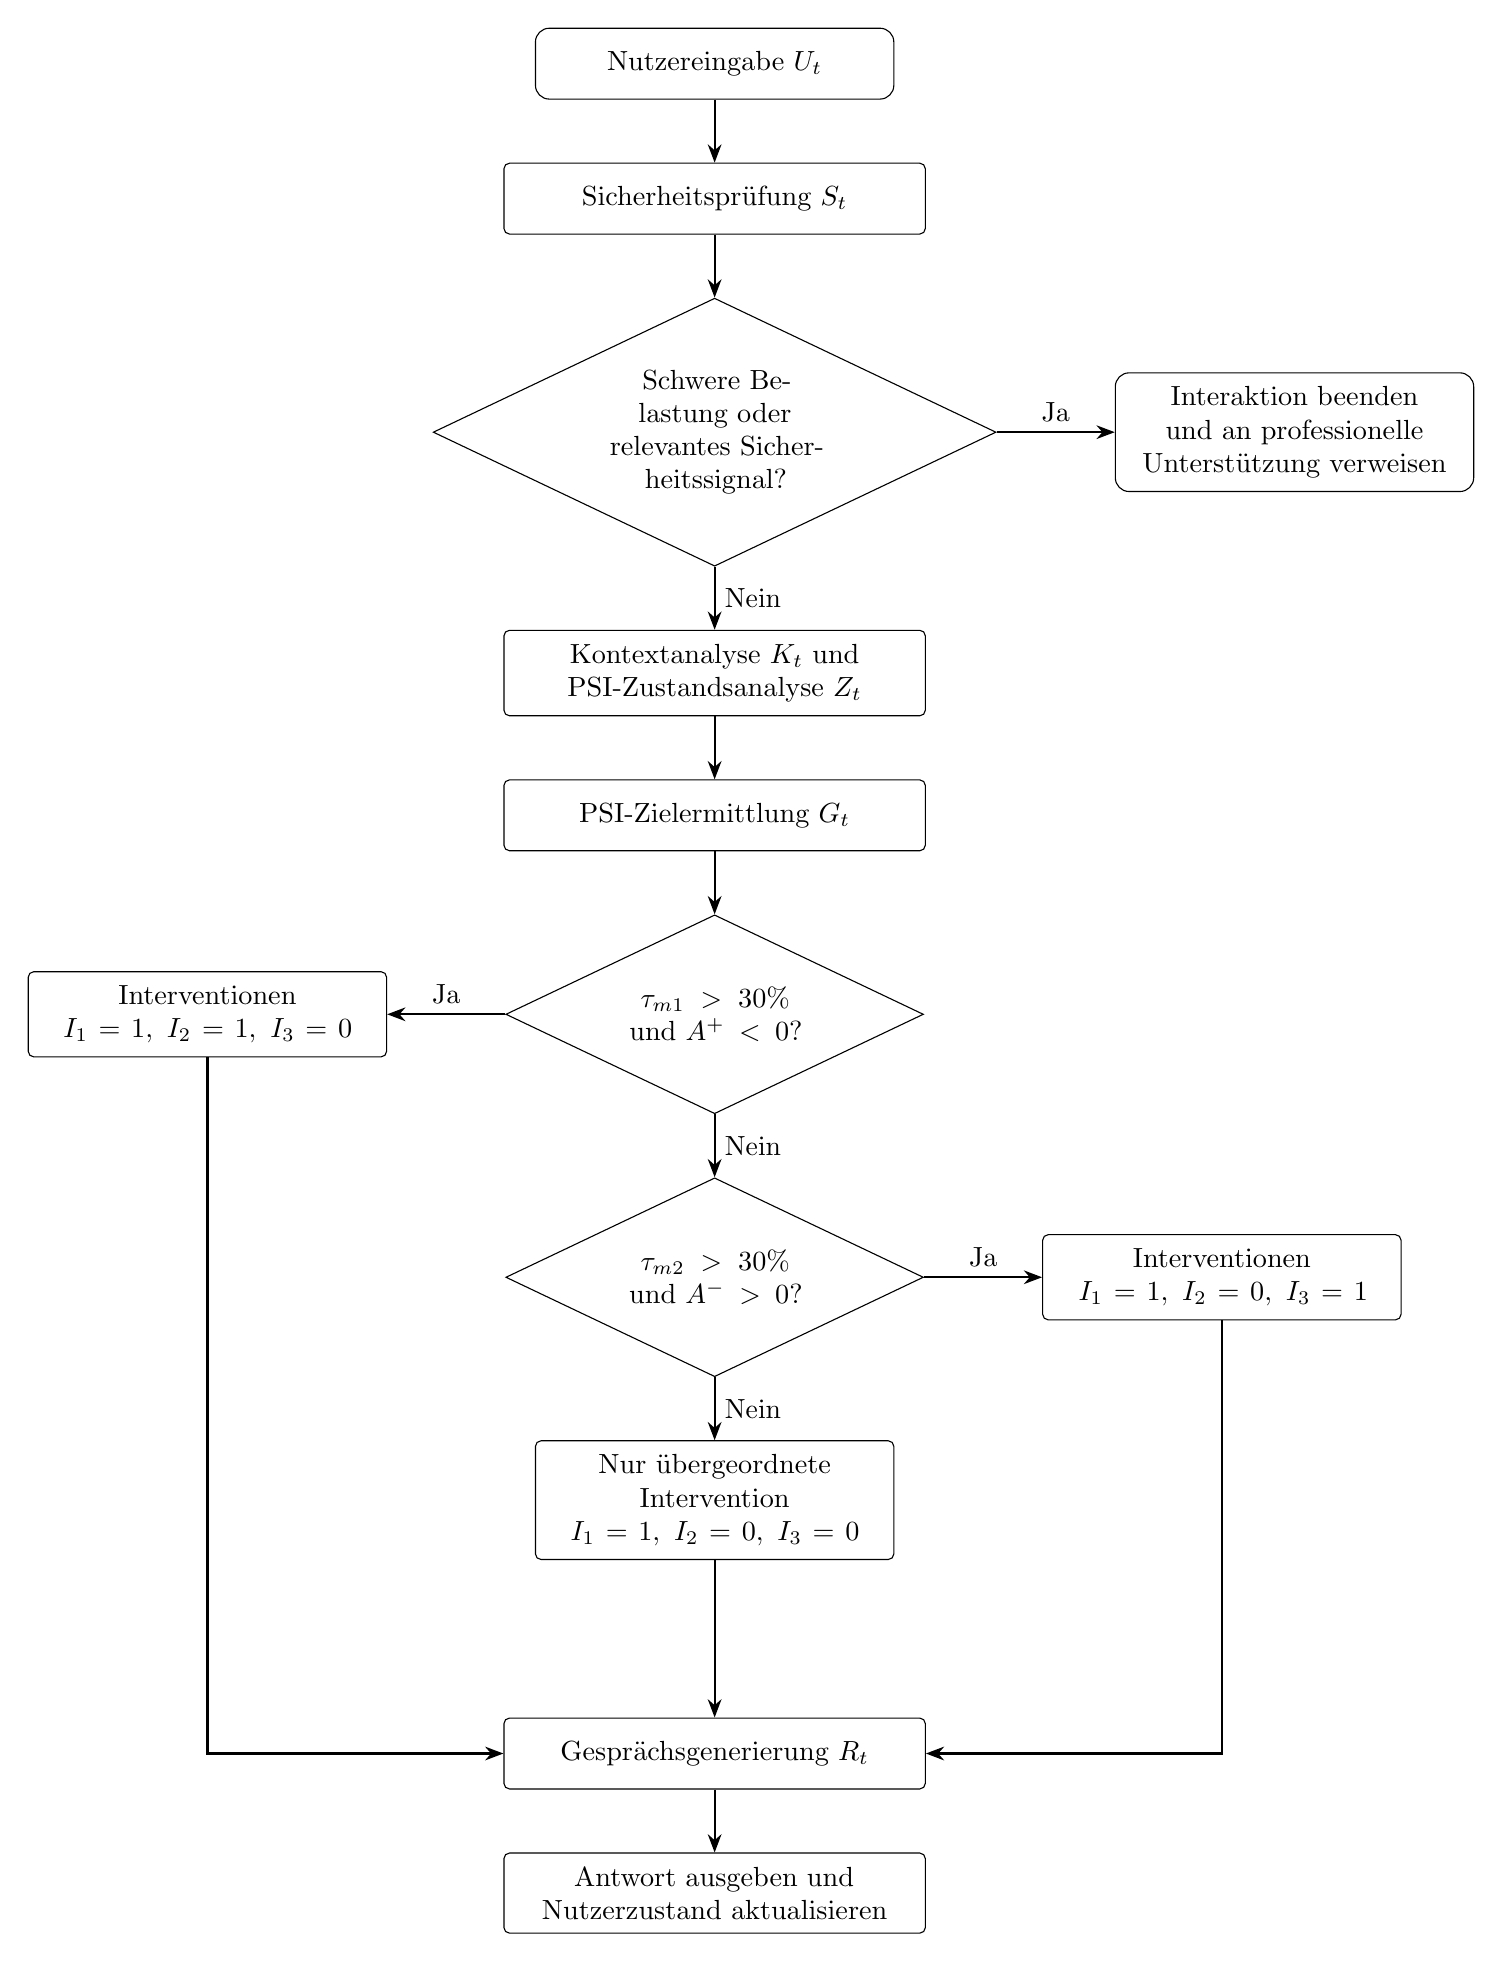
\begin{tikzpicture}[
    node distance=8mm and 15mm,
    >=Stealth,
    process/.style={
        rectangle, rounded corners=2pt,
        draw=black, align=center,
        text width=5.0cm, minimum height=9mm,
        inner sep=5pt
    },
    decision/.style={
        diamond, aspect=2.1, draw=black,
        align=center, text width=3.4cm,
        inner sep=2pt
    },
    terminal/.style={
        rectangle, rounded corners=5pt,
        draw=black, align=center,
        text width=4.2cm, minimum height=9mm,
        inner sep=5pt
    },
    intervention/.style={
        rectangle, rounded corners=2pt,
        draw=black, align=center,
        text width=4.2cm, minimum height=9mm,
        inner sep=5pt
    },
    line/.style={->, thick}
]

% Hauptablauf
\node[terminal] (start)
    {Nutzereingabe $U_t$};

\node[process, below=of start] (safety)
    {Sicherheitsprüfung $S_t$};

\node[decision, below=of safety] (risk)
    {Schwere Belastung oder\\
     relevantes Sicherheitssignal?};

\node[terminal, right=of risk] (stop)
    {Interaktion beenden\\
     und an professionelle\\
     Unterstützung verweisen};

\node[process, below=of risk] (context)
    {Kontextanalyse $K_t$ und\\
     PSI-Zustandsanalyse $Z_t$};

\node[process, below=of context] (goal)
    {PSI-Zielermittlung $G_t$};

% Interventionsentscheidungen
\node[decision, below=of goal] (checkI2)
    {$\tau_{m1}>30\%$ und $A^+<0$?};

\node[intervention, left=of checkI2] (onlyI1I2)
    {Interventionen\\
     $I_1=1,\ I_2=1,\ I_3=0$};

\node[decision, below=of checkI2] (checkI3)
    {$\tau_{m2}>30\%$ und $A^->0$?};

\node[intervention, right=of checkI3] (onlyI1I3)
    {Interventionen\\
     $I_1=1,\ I_2=0,\ I_3=1$};

\node[intervention, below=of checkI3] (onlyI1)
    {Nur übergeordnete Intervention\\
     $I_1=1,\ I_2=0,\ I_3=0$};

% Zusammenführung der drei Fälle
\node[process, below=20mm of onlyI1] (generation)
    {Gesprächsgenerierung $R_t$};

\node[process, below=of generation] (update)
    {Antwort ausgeben und Nutzerzustand aktualisieren};

% Verbindungen: Hauptablauf
\draw[line] (start) -- (safety);
\draw[line] (safety) -- (risk);

\draw[line] (risk.east) -- node[above, align=center]
    {Ja} (stop.west);

\draw[line] (risk.south) -- node[right]
    {Nein} (context.north);

\draw[line] (context) -- (goal);
\draw[line] (goal) -- (checkI2);

% Verbindungen: Interventionsauswahl
\draw[line] (checkI2.west) -- node[above]
    {Ja} (onlyI1I2.east);

\draw[line] (checkI2.south) -- node[right]
    {Nein} (checkI3.north);

\draw[line] (checkI3.east) -- node[above]
    {Ja} (onlyI1I3.west);

\draw[line] (checkI3.south) -- node[right]
    {Nein} (onlyI1.north);

% Zusammenführung der Interventionspfade
\draw[line] (onlyI1I2.south) |- (generation.west);
\draw[line] (onlyI1I3.south) |- (generation.east);
\draw[line] (onlyI1.south) -- (generation.north);

% Gesprächsverarbeitung und Rückkopplung
\draw[line] (generation) -- (update);

\end{tikzpicture}%
}
\caption{Entscheidungs- und Verarbeitungsablauf des PSI-basierten
Chatbot-Modells im traumasensiblen Coaching.}
\label{fig:psi-chatbot-ablauf}
\end{figure}


\section{Versuchsaufbau}
Grundlage des Versuchsaufbaus stellt ein experimentelles Design \citep{rubin2008comment} geppart mit einem Within-Scenario-Vergleich dar. Der Begriff und die Analyse wurde von \cite{eisenhardt2009building} geprägt und dient der inhaltlichen und kontextbezogenenen Analyse eines Szenarios beziehungsweise Fallbeispiels. Der aus dem Framework abgeleitete PSI-basierte Chatbot soll mittels Szenarien getestet werden. Dafür soll ein kontrollierter Vergleich zweier Chatbot-Varianten durchgeführt werden. Als Kontrollgruppe wird ein konventioneller LLM-Chatbot herangezogen und als Experimentalgruppe der PSI-basierte Chatbot. Beide Modelle erhalten den identischen Basis-Prompt, während der PSI-Chatbot zusätzlich die entwickelte PSI-Steuerungslogik erhält.

Der Versuchsaufbau dient dazu zu überprüfen, wie das PSI-basierte Chatbot-Modell im Vergleich zu einem konventionellen Chatbot funktioniert. Es werden die zwei experimentelle Bedingungen $B$ untersucht:
\begin{itemize}
    \item $B_{\text{Kontrolle}}(B_K)$: konventioneller Chatbot ohne PSI-basierte Dialogsteuerung
    \[U_t 
\rightarrow S_t
\rightarrow K_t
\rightarrow R_t\]
    \item $B_{\text{PSI}}(B_P)$: Chatbot auf Grundlage des entwickelten PSI-Modells
    \[U_t
\rightarrow S_t
\rightarrow K_t
\rightarrow Z_t
\rightarrow G_t
\rightarrow I_t
\rightarrow R_t
\]
\end{itemize}

mit:
\[
\begin{aligned}
U_t &:= \text{Nutzereingabe zum Zeitpunkt } t,\\
S_t &:= \text{Sicherheitsprüfung zum Zeitpunkt } t,\\
K_t &:= \text{Kontextanalyse zum Zeitpunkt } t,\\
Z_t &:= \text{PSI-Zustandsanalyse zum Zeitpunkt } t,\\
G_t &:= \text{Bestimmung des Unterstützungsziels zum Zeitpunkt } t,\\
I_t &:= \text{Auswahl der Intervention zum Zeitpunkt } t,\\
R_t &:= \text{generierte Chatbot-Antwort zum Zeitpunkt } t.
\end{aligned}
\]

Die beide Modelle bekommen dieselben Grundbedingungen. Für den Versuch wird das Modell gemini-3.8-flash herangezogen. Der Prompt beinhaltet für beide Bedingungen eine identisch definierte Sicherheitslogik, traumasensible Kommunikationsregeln, Coaching-Rolle und gleiche Nutzerinputs. Die beiden Modelle unterscheiden sich nur noch hinsichtlich der PSI-basierten Entscheidungslogik, bestehend aus PSI-Zustand, angestrebtem PSI-Ziel und Interventionsauswahl als Steuerungsmechanismus. Diese mehrstufige Entscheidungslogik dient somit als Kontrollvariable. 
Der Versuchsaufbau besteht aus 2 Szenarien, entsprechend der beiden Modulationsannahmen. 

\begin{enumerate}
    \item \textbf{Szenario 1 (Basisszenario $\mathcal{X}_{M1}$):} Bezug zur ersten Modulationsannahme (M1 - Willensbahnung)
    \item \textbf{Szenario 2 (Basisszenario $\mathcal{X}_{M2}$):} Bezug zur zweiten Modulationsannahme (M2 - Selbstentwicklung)
\end{enumerate}

Um die Funktionsweise der Chatbot-Modell ausreichend testen zu können, werden die Szenarien 100 mal durchlaufen und anschließend die Ergebnisse der beiden Bedingungen $B_{\text{Kontrolle}}$ und $B_{\text{PSI}}$ gegenübergestellt. 
Die formale Stichprobenarchitektur ist als ein $2 \times 2 \times 100$-faktorielles Design definiert (2 Modulationsannahmen $\times$ 2 experimentelle Bedingungen $\times$ 100 iterative Durchläufe). Daraus ergibt sich die Gesamtmenge der zu evaluierenden Datenzeilen ($N_{Total}$) wie folgt:

\begin{equation}
    N_{Total} = \left( 1\text{ Szenario}_{\mathcal{X}_{M1}} \times 100\text{ Iterationen} \times 2\text{ Bedingungen } [B_{PSI}, B_{K}] \right) 
\end{equation}
\begin{equation*}
    + \left( 1\text{ Szenario}_{\mathcal{X}_{M2}} \times 100\text{ Iterationen} \times 2\text{ Bedingungen } [B_{PSI}, B_{K}] \right) = 400\text{ Datenzeilen}
\end{equation*}


\subsection{Technische Umsetzung}

Um den theoretisch hergeleiteten Versuch über insgesamt $N = 400$ Simulationsläufe hinweg systematisch zu vergleichen, wurde eine programmgesteuerte Prüfumgebung in der Programmiersprache Python implementiert. 

Auf diese Weise wird sicher gestellt, dass jeder einzelne Simulationsdurchlauf isoliert betrachtet wird, um kontextuelle Verzerrungen innerhalb des Sprachmodells auszuschließen. Zu diesem Zweck wird bei jeder Iteration ein frischer API-Aufruf generiert, welcher das System-Prompt der jeweiligen experimentellen Bedingung ($B_{PSI}$ bzw. $B_K$) mit dem identischen, statischen Nutzer-Eingabetext ($U_t$) des entsprechenden Basisszenarios kombiniert.

\subsubsection{Ausgewähltes Sprachmodell: Gemini}

Für die Durchfühung des Experiments wird das Sprachmodell Gemini-3.8-flash von Google verwendet. Das Modells liefert eine hohe Performanz bei der Verarbeitung detaillierter System-Anweisungen und zeigt hohe Effizienz. Über das offizielle Google GenAI SDK lässt sich das Modell direkt in das Python-Skript einbinden.

Um eine hinreichende sprachliche und stochastische Varianz in den Ausgaben des Modells zu gewährleisten, ohne die strukturelle Einhaltung der deterministischen Verarbeitungs-Pipeline zu gefährden, wird der Modell-Parameter Temperatur gesetzt:
\begin{equation}
    \text{Temperature} = 0{,}7
\end{equation}

\subsubsection{Erstellung des Ergebnis-Datensatzes}

Da die Rohausgabe eines Large Language Models standardmäßig als unstrukturierter Freitext vorliegt, wurde ein zweistufiges Sicherungsverfahren implementiert, um die qualitativen Coaching-Dialoge von den quantitativen systemdiagnostischen Metriken sauber zu trennen. Der System-Prompt steuert die internen Berechnungen und Klassifikationen nach einem strikten XML-Schema. 
Das in Python implementierte Skript greift nach jedem erfolgreichen API-Call auf die Rohantwort des Modells zu und extrahiert diese Zeile. Im Ergebnis entsteht entsteht ein relationaler Datensatz mit 400 Datenzeilen.


\subsection{Sicherheitsprüfung}

Die Sicherheitsprüfung bildet nach der Nutzereingabe die zweite Ebene des Systems und orientiert sich an den NICE-Leitlinien \citep{kendrick2012common}. Sie stellt somit ein wichtiges Designprinzip des entwickleten Frameworks dar, welches für beide geprüften Bedingungen herangezogen wird. Ziel dieser Ebene ist es, anhand der Nutzereingabe eine strukturierte Bewertung der psychischen Belastung vorzunehmen und potenzielle Sicherheitssignale zu erkennen. Dabei wird zwischen milden, moderaten und schweren Belastungszuständen unterschieden.
Bei einer milden oder moderaten Belastung wird die Interaktion mit der anschließenden PSI-Zustandsanalyse fortgesetzt. Wird hingegen eine schwere Belastung beziehungsweise ein relevantes Sicherheitssignal erkannt, wird die weitere Verarbeitung durch das System beendet und der Nutzer an professionelle Unterstützung verwiesen. Die Sicherheitsprüfung dient somit insbesondere dazu, Situationen zu erkennen, in denen eine weitere Interaktion mit dem System nicht angemessen ist.

Für die strukturierte Einordnung werden mehrere Dimensionen berücksichtigt:

\begin{itemize}
    \item \textbf{Symptomatik:} gering / moderat / hoch
    \item \textbf{Dauer der Symptomatik:} kurz / länger andauernd
    \item \textbf{Alltagsbeeinträchtigung:} gering / deutlich / stark
\end{itemize}

Diese Kriterien werden dem Modell in strukturierter Form vorgegeben. Das LLM extrahiert auf Grundlage der Nutzereingabe die relevanten Merkmale und gibt diese als strukturierte Daten aus.
Das LLM stellt dabei keine medizinische Diagnose und klassifiziert keinen klinischen Zustand im diagnostischen Sinne. Stattdessen liefert es eine strukturierte Einschätzung der zuvor definierten Merkmale. Diese Einschätzung dient als Grundlage für die nachgelagerte regelbasierte Sicherheitslogik. Die eigentliche Entscheidung über die weitere Systemaktion erfolgt somit nicht ausschließlich durch das LLM, sondern durch explizit definierte Entscheidungsregeln. Dadurch soll insbesondere sichergestellt werden, dass sicherheitskritische Zustände nachvollziehbar und konsistent behandelt werden. Sind Symptomatik, Dauer und Alltagsbeeinträchtigung jeweils niedrig beziehungsweise kurz ausgeprägt, wird die Interaktion fortgesetzt.
Für einen schweren Belastungszustand greifen hingegen strengere Entscheidungsregeln. Werden beispielsweise eine hohe Symptomlast und eine starke Alltagsbeeinträchtigung festgestellt, wird der Zustand als schwer eingestuft und die Interaktion beendet. In diesem Fall erfolgt eine Weiterleitung an professionelle Unterstützung.
Die Sicherheitsprüfung fungiert damit als vorgeschaltete Kontrollinstanz. Während das LLM die aus der Nutzereingabe ableitbaren Merkmale strukturiert erfasst, bestimmen die explizit definierten Entscheidungsregeln die daraus resultierende Systemaktion. Die Trennung zwischen sprachmodellbasierter Merkmalsextraktion und regelbasierter Sicherheitsentscheidung erhöht dabei die Nachvollziehbarkeit und reduziert die Abhängigkeit von einer ausschließlich generativen Entscheidung des LLM.
Algorithmus \ref{alg:sicherheitspruefung_gesamt} stellt die regelbasierte Sicherheitsprüfung dar.

\begin{algorithm}[htbp]
\caption{Regelbasierte Logik der Sicherheitsprüfung ($S_t$)}
\label{alg:sicherheitspruefung_gesamt}
\begin{algorithmic}[1]
    \Statex \textbf{1. Strukturierte Merkmalsextraktion (Output des LLM):}
    \State \texttt{symptom\_burden} $\gets$ \texttt{moderate} \Comment{[low / moderate / high]}
    \State \texttt{duration} $\gets$ \texttt{long} \Comment{[short / long]}
    \State \texttt{functional\_impairment} $\gets$ \texttt{high} \Comment{[low / high]}
    \State \texttt{safety\_signal} $\gets$ \texttt{false} \Comment{[true / false]}
    \State \texttt{confidence} $\gets$ 0.86 \Comment{Statistische Sicherheit}
    
    \Statex
    \textbf{2. Regelbasierte Klassifizierung und Systemaktion:}
    \If{\texttt{safety\_signal} = \texttt{true} \textbf{or} (\texttt{symptom\_burden} = \texttt{high} \textbf{and} \texttt{functional\_impairment} = \texttt{high})}
        \State \texttt{risk\_level} $\gets$ \texttt{severe}
        \State \texttt{action} $\gets$ \texttt{professional\_support} \Comment{Pipeline stoppen, Hilfe verweisen}
        
    \ElsIf{\texttt{symptom\_burden} = \texttt{low} \textbf{and} \texttt{duration} = \texttt{short} \textbf{and} \texttt{functional\_impairment} = \texttt{low}}
        \State \texttt{risk\_level} $\gets$ \texttt{mild}
        \State \texttt{action} $\gets$ \texttt{continue} \Comment{Fahre mit Schritt 2 fort}
        
    \Else
        \State \texttt{risk\_level} $\gets$ \texttt{moderate}
        \State \texttt{action} $\gets$ \texttt{continue} \Comment{Fahre mit Schritt 2 fort}
    \EndIf
\end{algorithmic}
\end{algorithm}

\subsection{PSI-Zustands- und Potenzialanalyse}
Der Verscuh bezieht sich auf eine einzige initiale Eingabe des Nutzers in das System. Dieses Vorgehen wird gewählt, um einen möglichen Interpreatationsbias zu vermeiden. Dadurch lässt sich kein umfassendes Persönlichkeitsbild der Person, sondern ein für die aktuelle Situation spezifischer Zustand ableiten. Dies spiegelt einen klassischen Anwendungsfall wieder. Andieser Stelle sind meistens noch keine Informationen über den Nutzer bekannt.
Aus der Nutzereingabe wird basierend auf beobachteten Merkmalen eine regelgeleitete Hypothese des aktuellen Zustandes, in dem sich der Nutzer befindet, vorgenommen. Der Zustand soll dabei Rückschlüsse darauf geben, welches System im Sinne der PSI aktiv oder dominat ist. Die damit verbundene Potenzialanalyse liefert zusätzlich Informationen darüber, welches Entwicklungspotenzial bei dem Nutzer zu vermuten ist. Die Analyse wird basierend auf den vier Makrosystemen der PSI-Theorie, sowie der 7 Systemebenen der daruf basierenden Entwicklungsorientierten Osnabrücker Systemdiagnostik (EOS) durchgeführt \citep{kuhl2005neue,kuhl2004systemdiagnostik}. Diese ergeben entsprechend die psychologischen Dimensionen. Bei der EOS werden verschiedene Funktionsbereiche der Persönlichkeit betrachtet, welche sie gegenüber anderen Ansätzen hervorhebt. Es wird zwischen der Erstreaktion, welche spontane Eigenschaften und Verhaltensweisen beschreibt, und der Zweitreaktion, die motivationale und selbstregulatorische Kompetenzen der Person abbildet, unterschieden.

\subsubsection{Analyse des Zustandes mittels Erstreaktion}
Durch Analyse der Ebenen 1 bis 3 der EOS wird die Erstreaktion des Nutzers bewertet und damit eingeordnet, in welchem Zustand sich dieser befindet. Das System misst den vorherschenden biologischen Zustand des Nutzers.

\begin{itemize}
    \item \textbf{Ebene 1: Automatisches Verhalten:} Das Sytem analysiert das automatische Verhalten, dass heißt, wie spontan und reizgesteuert die Eingabe getätigt wurde.
    \item \textbf{Ebene 2: Temperament:} An dieser Stelle wird die Erregbarkeit und Aktivierung der Person gemessen.
    \item \textbf{Ebene 3: Affekte und Anreize:} Mittels zweidimensionaler Sentiment-Analyse wird gemessen, welche Emotionen vorherrschen.
\end{itemize}

\subparagraph{Operationalisierung der Affektbilanz}
Entsprechend der PSI-Theorie werden die Makrosysteme durch Affekte moduliert. Mittels Sentiment-Analyse wird der Text hinsichtlich der Affekte analysiert \citep{pang2008opinion}. Dabei werden zwei unterschiedliche Dimensionen untersucht und jeweils auf einer Skala von -1 bis +1 bewertet. 

\begin{enumerate}
    \item Positiver Affekt (\(A+\)): Misst Energie, Freude, Begeisterung gegenüber Nüchternheit, Demotivation (\(A+\) gehemmt)
    \item Negativer Akkeft (\(A+\)): Misst Bedrohung, Angst, Frust, Sorge gegenüber Gelassenheit, Sicherheit (\(A-\) herabreguliert) 
\end{enumerate}

Auf der Skala ergibt sich dann eine Tendenz für \(A+\) von -1.0 (völlig gehemmt/demotiviert) bis +1.0 (hochbegeistert/aktiviert) und für \(A-\) von -1.0 (völlig gelassen/sicher) bis +1.0 (hoher Frust/Angst/Sorge). Auf diese Weise ergibt sich ein zweidimensionales Affektsystem, das beachtet, das positive und negative Emotionen auch parallel existieren können.

\subsubsection{Analyse des Potenzials mittels Zweitreaktion}
Die Ebenen 4 bis 7 der EOS liefern Indikatioren hinsichtlich der Zweitreaktion der Person und damit des vorherschenden Entwicklungspotenzials. An dieser Stelle wird die kognitive Steuerungsfähigkeit des Nutzers analysiert. Im Zusammenspiel mit dem emotionalen Zustand und der Erstreaktion ergibt sich das Potenzial des Nutzers.

\begin{itemize}
    \item \textbf{Ebene 4: Stressbewältigung (Progression vs. Regression):} Analysiert, ob der Nutzer ein Problem (OES) nennt und dennoch zuversichtlich auf die Gesamtsituation (EG) blickt. Wenn ja, ist das Potenzial zur Progression hoch. Verharrt dieser jedoch im Problem, liegt eine Regression vor.
    \item \textbf{Ebene 5: Motive:} Das System filtert das übergeordnete Motiv hinsichtlich Anerkennung, messbaren Zielen, Autonomie oder Macht. Das Erkennen des Motivs zeigt das Ressourcen-Potenzial.
    \item \textbf{Ebene 6: Denken und Fühlen:} Es wird analysiert, wie der Nutzer sein Problem strukturiert. Nutzt er isoliert den Verstand (IG: „Ich muss funktionieren“) oder bettet er es in sein integratives Selbstwissen ein (EG: „Ich weiß aus Erfahrung, dass…“).
    \item \textbf{Ebene 7: Selbststeuerung:} Das System analysiert den Text gezielt nach Kontrollstrukturen und bewertet somit das Potenzial des Nutzers hinsichtlich Selbstregulation und Selbstmotivierung.
\end{itemize}

\subparagraph{Operationalisierung der aktiven Systeme}
Die 7 Systemebenen werden mittels linguistischer Merkmale analysiert und anhand eines Scores von 0 bis 3 bewertet. Diese Scores werden für das Modell als konkrte Bewertungslogik herangezogen.

\begin{itemize}
    \item \textbf{Score 0:} kein erkennbarer Hinweis
    \item \textbf{Score 1:} schwacher Hinweis
    \item \textbf{Score 2:} deutlicher Hinweis
    \item \textbf{Score 3:} sehr deutlicher Hinweis
\end{itemize}

Die psychischen Systeme stehen nach der PSI-Theorie in Wechselwirkung miteinander. Einzelne sprachliche Merkmale können daher auch mehreren Systemen zugeordnet werden.
Allgemeine Empathie und positive Formulierungen gelten nicht automatisch als PSI-Indikatoren. Entscheidend für die Bewertung ist die inhaltliche Funktion einer Formulierung, nicht allein ihre positive Tonalität.
Die Bewertung der dritten Ebene als besonders relevanter und desshalb separat ausgewiesenes Kriterium wurde bereits beschreiben. In Tabelle \ref{tab:psi_eos_ebenen_parser} ist die Klassifizierung der Ebenen 1 bis 7 dargestellt.

\begin{table}[htbp]
\centering
\small
\renewcommand{\arraystretch}{1.3}
\begin{tabularx}{\textwidth}{l p{2.2cm} X l}
\hline
\textbf{EOS-Systemebene} & \textbf{Aktives System} & \textbf{Linguistisches Merkmal (Indikator im Text)} & \textbf{Score} \\
\hline

\multirow{2}{*}{\textbf{E1: Gewohnheit}} 
& \textbf{IVS} & Verwendung von Alltagsfloskeln, Redewendungen, starre S-P-O-Sätze. & 0--3 \\
& \textbf{IG / OES} & Bruch von Verhaltensroutinen, stockende, unnatürliche Satzstrukturen. & 0--3 \\
\hline

\multirow{2}{*}{\textbf{E2: Temperament}} 
& \textbf{OES / IVS} & Hohe Erregung: Multiple Satzzeichen (?!), Großschrift, Interjektionen. & 0--3 \\
& \textbf{IG / EG} & Niedrige Erregung: Nüchterner, sachlicher Tonfall, fließende Syntax. & 0--3 \\
\hline

\multirow{2}{*}{\textbf{E4: Stressbewältigung}} 
& \textbf{EG} (Progression) & Syntaktische Kontrastierung („...aber ich weiß, dass es klappt“). & 0--3 \\
& \textbf{OES} (Regression) & Starres Verharren in der Problem- und Barrierenbeschreibung. & 0--3 \\
\hline

\multirow{2}{*}{\textbf{E5: Basismotive}} 
& \textbf{IG} & Leistungsmotiviert: „Ziele“, „Erfolg“, „besser werden“, „optimieren“. & 0--3 \\
& \textbf{OES} & Macht/Kontrollmotiviert: „Einfluss“, „Kontrolle“, „Sicherheit“, „Gefahr“. & 0--3 \\
& \textbf{IVS} & Anschlussmotiviert: „Team“, „Zusammenarbeit“, „Gemeinschaft“. & 0--3 \\
& \textbf{EG} & Freiheitsmotiviert: „Autonomie“, „unabhängig“, „ich selbst sein“. & 0--3 \\
\hline

\multirow{2}{*}{\textbf{E6: Kognition}} 
& \textbf{IG} & Analytisch: Deontische Modalverben (müssen/sollen), Wenn-Dann-Logik. & 0--3 \\
& \textbf{OES} & Defizitär: Hohe Frequenz von lexikalischen Negationen (nicht/kein). & 0--3 \\
& \textbf{EG} & Holistisch: Integrative Substantive („Zusammenhang“, „Erfahrung“). & 0--3 \\
& \textbf{IVS} & Pragmatisch: Dynamische Aktions-Verben im Präsens (machen/starten). & 0--3 \\
\hline

\multirow{2}{*}{\textbf{E7: Selbststeuerung}} 
& \textbf{EG} (Selbstregulation) & Metakognitive Verben („ich bemerke, dass ich gerade wütend bin“). & 0--3 \\
& \textbf{IG} (Selbstkontrolle) & Volitionale Disziplinphrasen („ich zwinge mich dazu, das zu tun“). & 0--3 \\
\hline

\end{tabularx}
\caption{Chronologischer Evaluations-Parser: Linguistische Zuordnung der aktiven Makrosysteme auf den einzelnen EOS-Ebenen inklusive Gewichtung (Scores 0--3).}
\label{tab:psi_eos_ebenen_parser}
\end{table}

Um aus den verbleibenden sechs Systemebenen ($E_1, E_2, E_4, E_5, E_6, E_7$) die relative Dominanz der vier psychischen Makrosysteme ($IG, OES, EG, IVS$) mathematisch abzuleiten, wird ein gewichtetes Aggregationsverfahren angewendet. Dieses verläuft in zwei sequentiellen Schritten:

\paragraph{Schritt A: Ermittlung der Rohpunkte ($R$)}
Das Large Language Model (LLM) evaluiert die Texteingabe Ebene für Ebene und vergibt für das dort als primär aktiv identifizierte Makrosystem einen diskreten Erkennungs-Score ($s \in \{0, 1, 2, 3\}$). Makrosysteme, die auf einer spezifischen Ebene keine linguistischen Marker aufweisen, werden für diese Ebene mit dem Wert $0$ codiert. Die totale Rohpunktzahl ($R_{\text{System}}$) eines Makrosystems ergibt sich folglich aus der Summe seiner Scores über alle sechs betrachteten Ebenen:
\begin{equation}
    R_{\text{System}} = \sum_{\text{Ebene} \in \{1,2,4,5,6,7\}} s_{(\text{Ebene}, \text{System})}
\end{equation}

\paragraph{Schritt B: Relative Normalisierung (Prozentuierung)}
Damit die Summe aller vier Makrosysteme in der Gesamtbetrachtung exakt $100\,\%$ ergibt, was eine zwingende mathematische Voraussetzung für die nachfolgenden Diskrepanz-Formeln zur Willenshemmung und gehemmten Selbstentwicklung darstellt, werden die Rohpunkte ins Verhältnis zur Gesamtsumme aller im Text vergebenen Punkte gesetzt:
\begin{equation}
    \%_{\text{System}} = \left( \frac{R_{\text{System}}}{R_{\text{IG}} + R_{\text{OES}} + R_{\text{EG}} + R_{\text{IVS}}} \right) \times 100
\end{equation}

Die Gewichtung der Systeme beinhaltet somit sowohl den aktuell aktiven Zustand (Erstreaktion) der Person, sowie auch ihr Potenzial zur persönlichen Entwicklung (Zweitreaktion). Durch Ebene 3 wird folglich zustätzlich der affektive Zustand berücksichtigt, um ein ganzheitliches Bild der spezifischen Situation zu erhlaten und darauf basierend ein geeignetes Coaching Ziel festzulegen.


\subsection{PSI-basierte Ziele}
Im Rahmen des traumasensiblen Coachings wird das übergeordnete Ziel verfolgt, eine Unterstützung zur Emotionsregulation, Stressbewältigung, Ressourcenaktivierung und Selbstregulation zu leisten \citep{kuhl2005neue}. Das Modell soll als reflektierendes KI-System dazu beizutragen, den Zugang zum Selbstsystem zu unterstützen, Selbstmotivation und Selbstberuhigung zu fördern, sowie die Entwicklung selbstkonguenter Ziele zu ermöglichen.
Die Ableitung des psychologischen Ziels sowie die Bestimmung des anzustrebenden Systemwechsels basieren auf den zwei zentralen Modulationsannahmen der PSI-Theorie \citep{Kuhl2000The}. Diese Annahmen zeigen, dass die Interaktion zwischen den kognitiven Makrosystemen nicht direkt, sondern über die Herauf- oder Herunterregulierung von positivem ($A+$) und negativem Affekt ($A-$) gesteuert wird.

\subsubsection{Regelbasierte Zielermittlung über die Modulationskanäle}
Die mathematische Grundlage bildet eine prozentuale Gewichtung der vier Makrosysteme durch das LLM, wobei gilt: $IG + OES + EG + IVS = 100\,\%$. Im Zusammenspiel mit den Werten der Affektbilanz ($A+$ und $A-$ im Intervall $[-1.0; +1.0]$) werden zwei Metriken definiert, dieie das Potenzial des Nutzers messbar machen:

\begin{enumerate}
    \item \textbf{Willensbahnung (Inkongruenz auf der $A+$-Achse):} 
    Eine Willenshemmung liegt vor, wenn der Nutzer eine hohe kognitive Absicht formuliert, jedoch nicht über den notwendigen positiven Affekt verfügt, um diese in Handlung zu übersetzen.
    \begin{equation}
        \text{Willenshemmung} = IG - IVS \quad \text{bei gleichzeitigem } A+ \le 0.0
    \end{equation}
    Ein hoher positiver Differenzwert indiziert, dass das Potenzial zur Verhaltensumsetzung blockiert ist.
    
    \item \textbf{Selbstentwicklung (Inkongruenz auf der $A-$-Achse):}
    Eine Hemmung der Selbstentwicklung liegt vor, wenn das Objekterkennungssystem durch unregulierten negativen Affekt dominiert wird, ohne dass das Extensionsgedächtnis zur Selbstberuhigung beitragen kann.
    \begin{equation}
        \text{Gehemmte Selbstentwicklung} = OES - EG \quad \text{bei gleichzeitigem } A- \ge 0.0
    \end{equation}
    Ein hoher positiver Differenzwert indiziert, dass das Potenzial zur Selbstberuhigung und ganzheitlichen Problemlösung blockiert ist.
\end{enumerate}

Auf Basis diesen Potenzials ergeben sich zwei Zielzustände entsprechend der Modulationsannahmen. Liebt eine Willenshemmung vor, wird eine Aktivierung des IVS angestrebt. Bei gehemmter Selsbtentwicklung steht eine Aktivierung des EG im Fukus.

\section{Intervention}
Der Steuerungsmechanismus stellt die regelbasierte Gesprächsinstanz dar, die entscheidet, welche Intervention ausgewählt wird und die Auswahl an den Gesprächsverlauf anpasst. Intervention meint in Abgrenzung dazu, eine konkrete Maßnahme bzw. Methode, die im Dialog eingesetzt wird. Nach dem bestehenden DTx-Modell wird eine Intervention anhand mehrerer Komponenten beschrieben. Die Komponenten sind: Therapieeinheit, Interventionseinheit, Entscheidungslogik, narrative Ebene, Unterstützungsfunktion und therapeutische Gesprächsinstanz. Der Steuerungsmechanismus ist eine technische Komponente des Modells. Er übernimmt die Funktion einer Entscheidungs- bzw. Auswahlinstanz. Es wird ausgewählt, welches Unterstützungsziel verfolgt werden soll, welche Interventionen grundsätzlich geeignet wären und welche davon also priorisierte Wahl herangezogen wird. Der zusätzliche Bestandteil an dieser Stelle ist die Berücksichtigung des aktuellen PSI-Zustands, sowie die Ableitung eines PSI-Ziels und die daraus resultierende Gewichtung geeigneter Interventionen. Im Sinne der PSI Theorie wird ein Wechsel der Systeme und damit die Veränderung des Zustandes vorrangig durch Regulation von Affekten und damit der emotionalen Steuerung von Verhalten bedingt \citep{Kuhl2000The}.

\paragraph{Intervention 1 ($I_1$): Übergreifende Haltung}
Es gibt einige Kriterien, die im Sinne der PSI Theorie übergreifend gelten sollen, damit eine traumasensible Persönlichkeitsentwicklung unterstützt werden kann. Diese Kriterien gelten auch dann, wenn die Indikatoren der beiden Modulationsannahmen nicht gegeben sind. 
Das Konzept der emotionalen Dialektik stellt als übergreifende Haltung im traumasensiblen Coaching-Kontext eine besondere Wichtigkeit dar. Demnach sollte ein Coach in dem Bewusstsein egieren, dass weder eine dauerhaft positive noch eine dauerhaft negative Stimmung entwicklungsfördernd ist. Der Klient soll dabei unterstützt werden, Emotionen funktional einzuordnen, sich nicht in affektiven Zuständen zu verlieren, sondern Gefühle flexibel zu verarbeiten und als motivationale Kraftquellen zu nutzen \citep{kuhl2005neue}. 

Folgende Kernaspekte ergeben sich aus dieser Beschreibung zur Entwicklung der Selsbtkompetenz:
\begin{itemize}
    \item $a_1$ := Emotionale Dialektik: flexibler Wechsel zwischen positiven und negativen Emotionen
    \item $a_2$ := Zeigen von Verständnis
    \item $a_3$ := Unterstützung selbstregulatorischer Prozesse
   \end{itemize}

In Kapitel \ref{prozess} ist die Bedeutung der Modulationsannahmen für Coachingprozesse beschreiben worden. Basierend auf den berechneten Kennzahlen ermittelt das System modulationsbasierte Interventionen:


\paragraph{Intervention 2 ($I_2$): Selbstmotivierung
(Modulationsannahme 1)}

An dieser Stelle wird der Übergang vom Intentionsgedächtnis
($IG$) zur intuitiven Verhaltenssteuerung ($IVS$) reguliert.
Die Intervention wird eingesetzt, wenn folgende Bedingungen
erfüllt sind:
\[
\text{Willenshemmung} > \tau
\quad \text{und} \quad A^+ < 0.0,
\]
wobei $\tau$ einen empirischen Schwellenwert bezeichnet,
z.\,B. $30\,\%$.

Das Coaching-Ziel besteht darin, den Klienten durch
Selbstmotivierung zur Umsetzung seiner Ziele zu befähigen.
Durch die Generierung positiver Affekte ($A^+ \uparrow$)
kann die Hemmung zwischen $IG$ und $IVS$ reduziert werden.

Daraus ergeben sich drei Kernaspekte der Intervention:
\begin{itemize}
    \item $b_1$:= Bestärkung durch Motivation, Zuversicht
    und Ermutigung
    \item $b_2$:= Pendeltechnik: positive Vorstellung des
    Ziels, bewusste Auseinandersetzung mit Schwierigkeiten
    und anschließende erneute Aktivierung positiver Gefühle
    \item $b_3$:= Aktivierung persönlicher Ressourcen
\end{itemize}


\paragraph{Intervention 3 ($I_3$): Selbstberuhigung
(Modulationsannahme 2)}

Ziel ist es, den Übergang vom Objekterkennungssystem
($OES$) zum erfahrungsbasierten Extensionsgedächtnis
($EG$) zu unterstützen. Die Intervention wird eingesetzt,
wenn folgende Bedingungen erfüllt sind:
\[
\text{Hemmung der Selbstentwicklung} > \tau
\quad \text{und} \quad A^- > 0.0.
\]
Ziel ist die Aktivierung des integrativen Erfahrungswissens
($EG$) durch die Herabregulierung negativer Affekte
($A^- \downarrow$).

Daraus ergeben sich drei Kernaspekte der Intervention:
\begin{itemize}
    \item $c_1$:= Wahrnehmen und Benennen von Gefühlen
    \item $c_2$:= Emotionale Integration
    \item $c_3$:= Spiegelung der eigenen Werte und Bedürfnisse
\end{itemize}


\subsubsection{Auswahl der Interventionen}
Aus der Beschreibung ergibt sich die Interventionsmenge wobei die einzelnen Interventionen die aufgezeigten Aspekte beinhalten: 

\[ I_j = \{I_1, I_2, I_3\} \]
mit $I_1(a_1, a_2, a_3)$, $I_2(b_1, b_2, b_3)$ und $I_3(c_1, c_2, c_3)$.

Diese werden anschließend durch die sprachliche Ausgestaltung in die Chatbotantwort übersetzt. Als zentraler technischer Artefakt wird ein Entscheidungsbaum verwendet, um eine systematische Auswahl zu gewährleisten \citep{baumel2025more}. Dieser ist in Abbildung \ref{fig:entscheidungsbaum_interventionsmenge} dargestellt. Demnach wählt der PSI-basierte Chatbot die Intervention nach den vorher bestimmten Zuständen beziehungsweise des Potenzials des Nutzers aus. Als Intervention wird demnach die übergreifende Haltung für jede mögliche Chatkonversation ausgewählt. Diese Intervention stellt somit eine Konstante im Modell dar ($I_1$=1). Anschließend wird mittels einer Wenn-Dann-Funktion geprüft, ob die Indikation einer Modulationsannahme gilt. In diesem Fall wird dann die entsprechende Intervention ausgewählt. 


\begin{figure}[htbp]
    \centering
    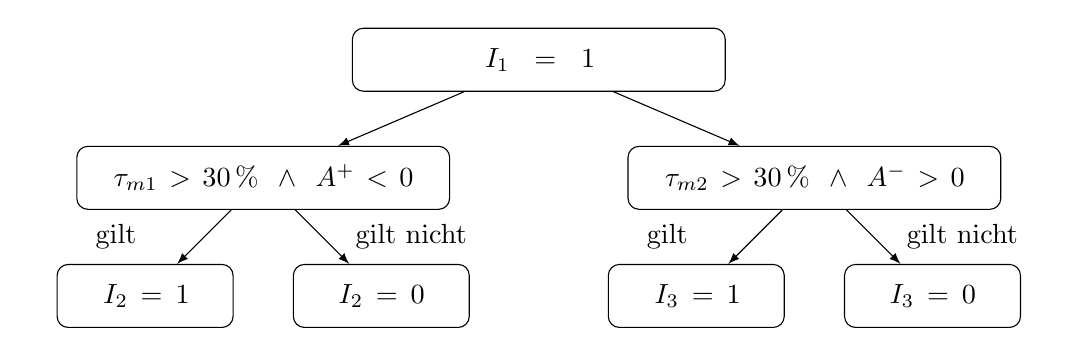
\begin{tikzpicture}[
        grow=down,
        level distance=1.5cm,
        every node/.style={
            draw,
            rounded corners,
            align=center,
            minimum height=0.8cm,
            text width=4.5cm
        },
        edge from parent/.style={draw, -latex},
        level 1/.style={
            sibling distance=7cm
        },
        level 2/.style={
            sibling distance=3cm,
            every node/.style={
                draw,
                rounded corners,
                align=center,
                minimum height=0.8cm,
                text width=2cm
            }
        }
    ]

    \node {$I_1 = 1$}
        child {
            node {$\tau_{m1} > 30\,\% \;\wedge\; A^+ < 0$}
            child {
                node {$I_2 = 1$}
                edge from parent
                node[left, draw=none] {gilt}
            }
            child {
                node {$I_2 = 0$}
                edge from parent
                node[right, draw=none] {gilt nicht}
            }
        }
        child {
            node {$\tau_{m2} > 30\,\% \;\wedge\; A^- > 0$}
            child {
                node {$I_3 = 1$}
                edge from parent
                node[left, draw=none] {gilt}
            }
            child {
                node {$I_3 = 0$}
                edge from parent
                node[right, draw=none] {gilt nicht}
            }
        };

    \end{tikzpicture}
    \caption{Entscheidungsbaum zur Bestimmung der Interventionsmenge $I_j$}
    \label{fig:entscheidungsbaum_interventionsmenge}
\end{figure}


Entsprechend des DTx-Modells würde die Therapieeinheit als Komponente dann verschiedene Interventionen und Gesprächsschritte bündeln, sodass ein unterstützender Prozess entsteht. Die narrative Ebene sorgt für einen nachvollziehbaren Gesprächsverlauf und liefert Motivation, Feedback, Erinnerungen, sowie technische Unterstützung. Die therapeutische Gesprächsinstanz erstellt dann die eigentliche Gesprächsebene des Chatbots.


\section{Gesprächsebene}

Die Gesprächsebene bildet die finale Instanz des entwickelten Frameworks und steuert die sprachliche Synthese der Chatbot-Antwort ($R_t$) zum Zeitpunkt $t$. Diese Ebene unterscheidet sich grundlegend zwischen den beiden experimentellen Bedingungen des Versuchsaufbaus: Während die Kontrollgruppe ($B_K$) eine rein reaktive, auf generischen traumasensiblen Coaching-Regeln basierende Antwort generiert, operiert die Experimentalgruppe ($B_{PSI}$) über eine mathematisch-psychologisch determinierte Verknüpfungslogik.

Für die Experimentalgruppe ($B_{PSI}$) wird das Large Language Model (LLM) mittels des System-Prompts dazu angewiesen, die Antwort nicht ausschließlich semantisch auf den Inhalt der Nutzereingabe ($U_t$) zu beziehen, sondern die zuvor berechneten Steuerungsvariablen exzessiv zu integrieren:
\[
R_t =
\begin{cases}
    \mathcal{G}(U_t,S_t,K_t), & B_K \\[6pt]
    \mathcal{G}(U_t,S_t,Z_t,G_t,I_t,K_t), & B_{PSI}
\end{cases}
\]
Dabei bezeichnet:
\[
\begin{aligned}
R_t &:= \text{generierte Chatbot-Antwort zum Zeitpunkt } t.\\
\mathcal{G} &:= \text{sprachliche Generierungsfunktion des LLM } t,\\
U_t &:= \text{Nutzereingabe zum Zeitpunkt } t,\\
S_t &:= \text{Ergebnis der Sicherheitsprüfung zum Zeitpunkt } t,\\
Z_t &:= \text{PSI-Zustandsanalyse zum Zeitpunkt } t,\\
G_t &:= \text{Unterstützungsziels zum Zeitpunkt } t,\\
I_t &:= \text{Auswahl der Intervention zum Zeitpunkt } t,\\
K_t &:= \text{Kontextanalyse zum Zeitpunkt } t,\\
\end{aligned}
\]
In diesem letzten Schritt wird erneut der Kontext der Interaktion herangezogen und bezüglich des auf EOS-Ebene 5 (\(K_{5t}\)) identifizierte unbewusste Basismotiv (Leistung, Macht, Anschluss oder Freiheit) interpretiert. An dieser Stelle wird geprüft, welche Metaphern, Schlüsselwörter und motivationalen Trigger das LLM wählt, um eine maximale Passung an die Persönlichkeitsstruktur des Nutzers zu erreichen. Die sprachliche Ausgestaltung wird dabei durch das Motivgerüst von $K$ eingefärbt. Ein leistungsmotivierter Nutzer wird über Zielerreichung und Optimierung adressiert, während ein freiheitsmotivierter Nutzer über Autonomie und Selbstbestimmung aktiviert wird. Durch diese strikte Trennung von Inhaltsebene (Nutzeranliegen) und Funktionsebene (PSI-Steuerung) wird sichergestellt, dass der Chatbot nicht lediglich bestehende, dysfunktionale Denkmuster reproduziert, sondern durch gezielte, motivkonforme Impulse zur aktiven Transformation beiträgt.


\section{Basispromt}



\section{Evaluation}
Das primäre Ziel der Evaluation besteht darin, die theoretisch-konzeptionelle Funktionsfähigkeit der modellierten Zustands-, Ziel- und Interventionslogik experimentell zu überprüfen. Es wird explizit keine klinische Wirksamkeitsstudie im therapeutischen Sinne durchgeführt. Vielmehr steht der Nachweis im Vordergrund, ob das Modell unter der Bedingung $B_{PSI}$ in der Lage is, ausgehend von einem initial erfassten Ausgangszustand eine theoriekonforme Intervention auszuwählen, die eine gerichtete, theoretisch fundierte Systemverschiebung auf den psychischen Achsen des Nutzers einleitet \citep{kuhl2005neue}. \\

Für jedes simulierte Interaktionsszenario wird der funktionale PSI-Zustand ($Z$) auf Basis der mathematischen Aggregationslogik zu zwei diskreten Messzeitpunkten evaluiert:
\begin{itemize}
    \item $Z_{t_0}$: Der empirische Ausgangszustand des Nutzers vor der Intervention, abgeleitet aus der relativen Normalisierung der initialen Nutzereingabe ($U_t$).
    \item $Z_{t_1}$: Der tatsächliche, phänomenologische Systemzustand, welcher durch die linguistische Analyse der generierten Chatbot-Antwort ($R_t$) induziert und direkt im Anschluss gemessen wird.
\end{itemize}

Im Rahmen des Systemtests generieren sowohl die Experimentalgruppe ($B_{PSI}$) als auch die Kontrollgruppe ($B_{K}$) auf Basis identischer Szenarien-Inputs eine Antwort $R_t$. Diese Antworten werden anschließend mittels der linguistischen Kriterien aus Tabelle \ref{tab:psi_eos_ebenen_parser} bewertet, um die Ausprägung des tatsächlichen Folgezustands $Z_{t_1}$ mathematisch zu bestimmen und den resultierenden Transformationseffekt im direkten Vorher-Nachher-Vergleich zu analysieren.

\subsection{Metriken und mathematische Operationalisierung}
Um die theoriegeleitete Transformation der funktionalen Systemzustände numerisch zu erfassen, wird kein statischer, numerischer Zielzustand vordefiniert. Die Evaluation fokussiert stattdessen die Überprüfung einer gerichteten Systemverschiebung (\textit{Directional Shift}) auf den theoretisch postulierten Systemachsen. Ein Zustand $Z$ zu einem beliebigen Messzeitpunkt wird über seine relativen Makrosystem-Scores ($\%System$) im vierdimensionalen Raum beschrieben.

Der experimentelle Steuerungseffekt wird direkt über das Differenzenmaß ($\Delta$) der normalisierten Prozentwerte zwischen dem Ausgangszustand ($Z_{t_0}$) und dem tatsächlichen Folgezustand ($Z_{t_1}$) operationalisiert:
\begin{equation}
    \Delta\%System = \%System(Z_{t_1}) - \%System(Z_{t_0})
\end{equation}

\subsubsection{Szenarienspezifische Zielmetriken nach Modulationsannahmen}
Die Erfolgskontrolle basiert auf der gerichteten Veränderung jener psychischen Systeme, die laut den Modulationsannahmen der PSI-Theorie durch die jeweilige Intervention aktiviert werden sollen:
\begin{enumerate}
    \item \textbf{Fokus Erste Modulationsannahme (Willensbahnung):} Das primäre Evaluationsziel bei vorliegender Willenshemmung ist die Aktivierung der Intuitiven Verhaltenssteuerung ($IVS$) zur Auflösung der Blockade des Intentionsgedächtnisses ($IG$). Der Steuerungseffekt ($E_{M1}$) bestimmt sich somit primär über den Zuwachs des IVS-Scores:
    \begin{equation}
        E_{M1} = \Delta\%IVS = \%IVS(Z_{t_1}) - \%IVS(Z_{t_0})
    \end{equation}
    
    \item \textbf{Fokus Zweite Modulationsannahme (Selbstentwicklung):} Das primäre Evaluationsziel bei vorliegender stressinduzierter Hemmung der Selbstentwicklung ist die Wiederherstellung des Selbstzugangs durch Aktivierung des Extensionsgedächtnisses ($EG$) zur Reduktion des fehlerfokussierten Objekterkennungssystems ($OES$). Der Steuerungseffekt ($E_{M2}$) bestimmt sich somit über den Zuwachs des EG-Scores:
    \begin{equation}
        E_{M2} = \Delta\%EG = \%EG(Z_{t_1}) - \%EG(Z_{t_0})
    \end{equation}
\end{enumerate}
Ein positiver Wert ($E > 0$) indiziert den theoriekonformen Systemwechsel, während ein Wert von $E \le 0$ ein Verharren in der dysfunktionalen Blockade oder eine Vertiefung der Problem-Regression signalisiert.

\subsection{Hypothesenformulierung und statistische Auswertung}
Der zentrale statistische Vergleich fokussiert nicht die absolute Qualität einzelner Dialogsequenzen, sondern die relative Überlegenheit der Interventionssteuerung unter der Bedingung $B_{PSI}$ gegenüber der Kontrollbedingung $B_{K}$. Geprüft wird, ob die mathematisch gesteuerte Experimentalgruppe zu einer signifikant stärkere Aktivierung des jeweils indizierten Zielsystems führt. Es werden die folgenden Forschungshypothesen aufgestellt:

\begin{equation}
    H_{1, M1}: E_{M1, B_{PSI}} > E_{M1, B_{K}} \quad \Longrightarrow \quad (\Delta\%IVS)_{B_{PSI}} > (\Delta\%IVS)_{B_{K}}
\end{equation}
\begin{center}
    \begin{minipage}{0.85\textwidth}
    \textit{Die Anwendung des PSI-basierten Modells ($B_{PSI}$) führt bei Szenarien zur ersten Modulationsannahme im Vergleich zu einer konventionellen Kontrollbedingung ($B_{K}$) zu einer signifikant stärkeren Aktivierung der Intuitiven Verhaltenssteuerung ($IVS$).}
    \end{minipage}
\end{center}

\begin{equation}
    H_{1, M2}: E_{M2, B_{PSI}} > E_{M2, B_{K}} \quad \Longrightarrow \quad (\Delta\%EG)_{B_{PSI}} > (\Delta\%EG)_{B_{K}}
\end{equation}
\begin{center}
    \begin{minipage}{0.85\textwidth}
    \textit{Die Anwendung des PSI-basierten Modells ($B_{PSI}$) führt bei Szenarien zur zweiten Modulationsannahme im Vergleich zu einer konventionellen Kontrollbedingung ($B_{K}$) zu einer signifikant stärkeren Aktivierung des Extensionsgedächtnisses ($EG$).}
    \end{minipage}
\end{center}

\vspace{2mm}
Die korrespondierenden Nullhypothesen ($H_0$) lauten dementsprechend:
\begin{align}
    H_{0, M1}: (\Delta\%IVS)_{B_{PSI}} \le (\Delta\%IVS)_{B_{K}} \\
    H_{0, M2}: (\Delta\%EG)_{B_{PSI}} \le (\Delta\%EG)_{B_{K}}
\end{align}
\begin{center}
    \begin{minipage}{0.85\textwidth}
    \textit{Die Anwendung des PSI-basierten Modells ($B_{PSI}$) führt im Vergleich zur Kontrollbedingung ($B_{K}$) zu keiner signifikant stärkeren Aktivierung des jeweils theoriekonformen Zielsystems ($IVS$ bzw. $EG$).}
    \end{minipage}
\end{center}

Da die durch das LLM vergebenen Erkennungs-Scores (Ebenen 1--7) ein ordinales Skalenniveau aufweisen und die berechneten Differenzenmaße ($\Delta\%System$) aufgrund des stochastischen Verhaltens von Sprachmodellen nicht als normalverteilt vorausgesetzt werden können, wird für den nicht-parametrischen Vergleich der verbundenen Stichproben der \textit{Wilcoxon-Vorzeichen-Rang-Test} herangezogen. Das statistische Signifikanzniveau für die Ablehnung der Nullhypothese wird auf einseitig $\alpha = 0{,}05$ festgelegt, bei einer Stichprobenarchitektur von exakt $n = 10$ verbundenen Paaren pro Modulationsannahme.

\subsubsection{Statistische Effektstärke ($r$)}
Ergänzend zur Prüfung des p-Werts wird die standardisierte Effektstärke $r$ berechnet, um die praktische Relevanz der Interventionssteuerung unabhängig vom Signifikanzniveau zu quantifizieren. Da es sich um ein nicht-parametrisches Verfahren handelt, wird $r$ aus der standardisierten Teststatistik $Z_{stat}$ des Wilcoxon-Tests abgeleitet:
\begin{equation}
    r = \frac{|Z_{stat}|}{\sqrt{N}}
\end{equation}
Hierbei entspricht $N = 10$ der Anzahl der Simulationspaare der jeweiligen Bedingungsgruppe. Die Interpretation der Effektstärke erfolgt nach den Schwellenwerten von Cohen: $r \ge 0{,}1$ indiziert einen schwachen, $r \ge 0{,}3$ einen mittleren und $r \ge 0{,}5$ einen starken experimentellen Steuerungseffekt.

    \chapter{Demonstration und Ergebnisse}

In diesem Kapitel wird die Funktionsfähigkeit des entwickelten PSI-Coaching-Frameworks anhand einer kontrollierten Dialogsimulation demonstriert. Ziel dieser Demonstration ist es, die Kette von der initialen Nutzereingabe ($U_{t_0}$) über die regelbasierte Zustandsbestimmung bis hin zur theoriegeleiteten Antwortgenerierung ($R_t$) empirisch zu untersuchen. Es wird demonstriert, wie die Experimentalgruppe ($B_{PSI}$) im direkten Vergleich zur Kontrollgruppe ($B_K$) auf ungesehene Fallbeispiele reagiert und ob eine gerichtete Systemverschiebung indiziert werden kann.

\section{Szenarienauswahl und theoriegeleitete Soll-Herleitung}

Für das kontrollierte Experiment wurden zwei Basisszenarien aus der Literatur adaptiert. Die Auswahl dieser spezifischen Szenarien erfolgte gezielt, da sie die beiden primären psychischen Blockadeformen der PSI-Theorie (Willenshemmung auf der $A^+$-Achse und Hemmung der Selbstentwicklung auf der $A^-$-Achse) operationalisieren. Diese Auswahl ermöglicht eine theoretische Soll-Herleitung des Ergebnisses. Dieser Herleitung wird in der Evaluation das Ergebniss des Chatbots gegenüber gestellt um zu prüfen, ob eine Systemverschiebung im Sinne der PSI-Theorie durch das LLM möglich ist.

\subsection{Szenario 1 (Basisszenario $\mathcal{S}_{M1}$): Der prokrastinierende Manager}
\paragraph{Beschreibung:} Ein 32-jähriger Abteilungsleiter berichtet im Coaching, in einer Sackgasse festzustecken. Die strategischen Ziele seien zwar klar definiert und er wolle sich unbedingt verbessern und die Prozesse optimieren, er müsse sich jedoch jeden Tag aufs Neue unter hohem Druck an den Schreibtisch zwingen und blockiere komplett. Seine Gedanken geraten ins Stocken, er bricht seine täglichen Verhaltensroutinen ab, prokrastiniert und erlebt ein intensives Gefühl der demotivierten, nüchternen Frustration. Er weiß theoretisch genau, was er tun soll, schafft es aber nicht, ins Handeln zu kommen \citep{kuhl2014psi}.

\paragraph{Theoretische Soll-Herleitung:} 
Die linguistische Analyse der Erst- und Zweitreaktionen (EOS) zeigt eine klassische Willenshemmung. Der Manager verfügt über ein hochaktives Intentionsgedächtnis (IG), welches sich in der permanenten Formulierung von Zielen ausdrückt (Ebene 6: analytisch; Ebene 7: Selbstkontrolle). Da jedoch der positive Affekt gehemmt ist ($A^+ < 0$), ist der Übergang in die Intuitive Verhaltenssteuerung (IVS) blockiert. Der Klient verharrt im unproduktiven Planen.
\begin{itemize}
    \item Ausgangszustand $Z_{t_0}$: Mathematische IG-Dominanz bei gehemmtem positiven Affekt ($A^+ < 0$). Der Diskrepanzwert überschreitet den Schwellenwert ($\tau_{m1} = \%IG - \%IVS > 15\%$).
    \item Psychologisches Unterstützungsziel $G$: Handlungsbahnung (Willensbahnung) durch Aktivierung des IVS durch Erzeugung positiver Affekte.
    \item Soll-Intervention $I_j$: Intervention $I_2$ (Affektive Pendeltechnik). Durch den gesteuerten Wechsel zwischen Zielvisualisierung, bewusster Barrierenanalyse und erneuter Ressourcenaktivierung soll die IVS re-aktiviert werden.
    \item Evaluationskriterium für den Folgezustand $Z_{t_1}$: Nachweis einer theoriekonformen, gerichteten Systemverschiebung hin zum Zielsystem, operationalisiert über einen messbaren Zuwachs des IVS-Scores ($E_{M1} = \Delta\%IVS > 0$).
\end{itemize}

\subsection{Szenario 2 (Basisszenario $\mathcal{S}_{M2}$): Die belastete Berufsschullehrerin}
\paragraph{Beschreibung:} Eine 41-jährige Berufsschullehrerin beschreibt im Coaching, unter anhaltendem Stress zu leiden, sich oft ziemlich erschöpft zu fühlen und klagt über psychosomatische Kopf- und Nackenschmerzen. Sie habe das Gefühl, im Alltag ständig in einem Hamsterrad zu laufen und finde selbst an Wochenenden oder in kurzen Pausen kaum noch echte Entspannung. Ihr Blick sei verengt und starr auf die Probleme, Barrieren und Gefahren gerichtet, sodass sie überall Fehler und Unstimmigkeiten entdecke. Ihr fehle momentan jede Orientierung, sie habe den Zugang zu den eigenen Bedürfnissen verloren und passe sich fast nur noch fremden Erwartungen an \citep{kuhl2014psi}.

\paragraph{Theoretische Soll-Herleitung:} 
Dieses Szenario operationalisiert eine stressinduzierte Hemmung der Selbstentwicklung. Durch den permanenten Stress ist der negative Affekt unreguliert hoch ($A^- > 0$). Dies führt zu einer Dominanz des Objekterkennungssystems (OES), welches sich im starren Verharren auf die Symptome, Fehler und das Gefühl des Gefangenseins äußert (Ebene 4: Regression; Ebene 6: defizitär). Der Zugriff auf Erfahrungswissen und die beruhigenden Ressourcen des Extensionsgedächtnisses (EG/Selbst) ist blockiert, was zu einer drohenden Selbstfiltration führt.
\begin{itemize}
    \item Ausgangszustand $Z_{t_0}$: Mathematische OES-Dominanz bei erhöhtem negativen Affekt ($A^- > 0$). Der Diskrepanzwert überschreitet den Schwellenwert ($\tau_{m2} = \%OES - \%EG > 15\%$).
    \item Psychologisches Unterstützungsziel $G$: Selbstberuhigung und Wiederherstellung des Selbstzugangs durch Herabregulierung des negativen Affekts ($A^- \downarrow$).
    \item Soll-Intervention $I_j$: Intervention $I_3$ (Achtsamkeitsbasierte Affektregulation und Selbstberuhigung). Durch emotionale und körperbezogene Selbstwahrnehmung, Benennung von Emotionen und das Verlangsamen der Situation muss die physiologische Erregung gedrosselt und das EG aktiviert werden.
    \item Evaluationskriterium für den Folgezustand $Z_{t_1}$: Nachweis einer theoriekonformen, gerichteten Systemverschiebung hin zum Zielsystem, operationalisiert über einen messbaren Zuwachs des EG-Scores ($E_{M2} = \Delta\%EG > 0$).
\end{itemize}

\section{Ergebnisse}

Im Folgenden werden die empirischen Ergebnisse der kontrollierten Dialogsimulation dargestellt und evaluiert. Das Ziel der statistischen Analyse bestand darin, die relative Überlegenheit der PSI-basierten Dialogsteuerungslogik (Bedingung $B_{PSI}$) gegenüber der konventionellen, rein traumasensiblen Kontrollbedingung ($B_K$) über einen Stichprobenumfang von insgesamt $N = 400$ Simulationsläufen (jeweils $n = 100$ verbundene Paare pro betrachteter Modulationsannahme) experimentell nachzuweisen. Die statistische Auswertung wurde mittels des einseitigen Wilcoxon-Vorzeichen-Rang-Tests bei einem Signifikanzniveau von $\alpha = 0{,}05$ durchgeführt.

\subsection{Deskriptive Statistik und Systemverschiebungen}

Die Auswertung der Richtungsverschiebungen zeigt für beide Szenariokonfigurationen eine theoriekonforme Tendenz zur Aktivierung der angestrebten Zielsysteme. Der Steuerungseffekt bestimmt sich über das Differenzenmaß:
\begin{equation}
    \Delta\%System = \%System(Z_{t_1}) - \%System(Z_{t_0})
\end{equation}
Tabelle \ref{tab:ergebnisse_uebersicht} fasst die deskriptiven Parameter und die inferenzstatistischen Kennwerte der beiden experimentellen Hauptachsen zusammen.

\begin{table}[htbp]
\caption{Übersicht der inferenzstatistischen Ergebnisse und Systemverschiebungen ($N=100$)}
\label{tab:ergebnisse_uebersicht}
\centering
\small
\setlength{\tabcolsep}{4pt} % Verringert den horizontalen Spaltenabstand für mehr Platz
% Feste Breiten für die Datenspalten schieben den maximalen Platz in die erste X-Spalte
\begin{tabularx}{\textwidth}{X *{2}{p{1.4cm}} *{3}{p{1.6cm}} p{1.3cm}}
\hline
\textbf{Zielachse (Modulationsannahme)} & \centering\textbf{$M_{PSI}$ (\%)} & \centering\textbf{$M_{K}$ (\%)} & \centering\textbf{Statistik ($W$)} & \centering\textbf{$Z_{stat}$} & \centering\textbf{$p$-Wert} & \centering\textbf{Effektst. ($r$)} \tabularnewline \hline
M1: Willensbahnung ($\Delta\%IVS$) & \centering $+24{,}05$ & \centering $+11{,}78$ & \centering $4753{,}0$ & \centering $+7{,}661$ & \centering $< 0{,}00001$ & \centering $0{,}766$ \tabularnewline
M2: Selbstentwicklung ($\Delta\%EG$) & \centering $+26{,}51$ & \centering $+21{,}72$ & \centering $3053{,}0$ & \centering $+1{,}815$ & \centering $0{,}01309$ & \centering $0{,}182$ \tabularnewline \hline
\end{tabularx}
\end{table}




    \chapter{Evaluation}

\subsection{Inferenzstatistische Prüfung der ersten Modulationsannahme (M1)}

Die erste Forschungshypothese $H_{1, M1}$ postulierte, dass die Anwendung des PSI-basierten Modells ($B_{PSI}$) im Kontext einer chronischen Willenshemmung zu einer signifikant stärkeren Aktivierung der Intuitiven Verhaltenssteuerung ($IVS$) führt als die konventionelle Kontrollbedingung ($B_K$). 

Der einseitige Wilcoxon-Vorzeichen-Rang-Test für verbundene Stichproben bestätigt diese Annahme. Die Experimentalgruppe erzielte eine mittlere positive Verschiebung des $IVS$-Scores von $M = +24{,}05\%$, während die Kontrollgruppe lediglich einen Zuwachs von $M = +11{,}78\%$ aufwies. Die inferenzstatistische Analyse weist eine hochsignifikante Abweichung von der Nullhypothese auf:
\begin{math}
    W = 4753{,}0; \ z = +7{,}661; \ p < 0{,}00001
\end{math}.

Die standardisierte Effektstärke nach Cohen beträgt $r = 0{,}766$. Gemäß den Schwellenwerten von Cohen (1988) indiziert dies einen starken experimentellen Steuerungseffekt. Die Nullhypothese $H_{0, M1}$ kann somit vollständig verworfen und die Alternativhypothese $H_{1, M1}$ als empirisch bestätigt angesehen werden. Die mathematische Konditionierung des Suchraums über die berechnete Diskrepanzvariable $\tau_{m1}$ führt zu einer hochgradig robusten und praxisrelevanten Handlungsbahnung.

\subsection{Inferenzstatistische Prüfung der zweiten Modulationsannahme (M2)}

Die zweite Forschungshypothese $H_{1, M2}$ untersuchte den Transformationseffekt bei vorliegender stressinduzierter Hemmung der Selbstentwicklung. Es wurde angenommen, dass die Bedingung $B_{PSI}$ eine signifikant stärkere Aktivierung des erfahrungsbasierten Extensionsgedächtnisses ($EG$) über Mechanismen der angeleiteten Selbstberuhigung bewirkt als die Bedingung $B_K$.

Deskriptiv verzeichneten beide Gruppen eine deutliche Erhöhung des holistischen Systemanteils. Unter der PSI-basierten Dialogsteuerung stieg der relative $EG$-Anteil im Mittel um $M = +26{,}51\%$, während unter der konventionellen Bedingung ein Zuwachs von $M = +21{,}72\%$ gemessen wurde. Der mathematische Paarvergleich bestätigt die statistische Überlegenheit des Interventionsmodells:
\begin{math}
    W = 3053{,}0; \ z = +1{,}815; \ p = 0{,}01309
\end{math}.

Da der p-Wert unter dem kritischen Schwellenwert von $\alpha = 0{,}05$ liegt, wird die Nullhypothese $H_{0, M2}$ ebenfalls verworfen und die Alternativhypothese $H_{1, M2}$ angenommen. Die standardisierte Effektstärke beträgt hierbei jedoch lediglich $r = 0{,}182$, was einem schwachen experimentellen Steuerungseffekt entspricht. 

Obwohl das System $B_{PSI}$ die theoriegeleitete Selbstberuhigung und die Integration in das Selbstsystem im Vergleich zur Kontrollgruppe statistisch nachweisbar verbessert, fällt die relationale Differenzierung auf dieser Achse experimentell deutlich geringer aus als auf der Handlungsbahnungsachse ($M1$). Dies deutet darauf hin, dass konventionelle, inhärent empathische traumasensible Kommunikationsmuster (Bedingung $B_K$) bereits eine starke basale Entlastung und damit eine implizite Herabregulierung des negativen Affekts bewirken, wodurch sich der zusätzliche translationale Effekt des mathematischen Regelwerks relativiert.


\section{Bewertung des Modells}
    \chapter{Diskussion und Implikationen}

\section{Theoretische und wissenschaftliche Einordnung}

\subsection{Erste Modulationsannahme M1 – Willensbahnung}
Aus theoretischer Perspektive lässt sich das Ergebnis zur ersten Modulationsannahme (Szenario $XM_1$) von \cite{Kuhl2000The} mit der gezielten Berücksichtigung der affektiven Ausgangslage und der daraus abgeleiteten Interventionen erklären. Die Ergebnisse haben an dieser Stelle einen positiven Effekt von 9,99 Prozentpunkten der Experimentalgruppe gegenüber der Kontrollgruppe gezeigt. Während $B_K$ primär auf eine allgemeine traumasensible Gesprächsführung zurückgreift, berücksichtigt $B_{PSI}$ zusätzlich die zuvor identifizierte Inkongruenz zwischen Intentionsgedächtnis und intuitiver Verhaltenssteuerung. 

Durch Interventionen wie Bestärkung, Pendeltechnik und Ressourcenaktivierung wird gezielt die Erzeugung positiver Affekte angestrebt. Die Ergebnisse deuten darauf hin, dass durch den Einsatz dieser Interventionen eine Verschiebung des untersuchten linguistischen Indikators in die erwartete Richtung erreicht werden kann. Diese Ergebnisse bestärken somit die einen förderlichen Einsatz der Pendeltechnik entsprechend \cite{kuhl2005neue} sowie dem Einsatz im menschlichen Coaching \citep{kuhl2014psi}. Die Interventionen lassen sich relativ klar in sprachliche Impulse übersetzen, was die Steuerung und Verwendung im Modell erleichtert. An dieser Stelle sollte jedoch kritisch beleuchtet werden, dass die Ergebnisse vorrangig eine Veränderung linguistischer Indikatoren und nicht die tatsächliche Aktivierung der psychischen Systeme beim Menschen belegen. Es kann keine Aussage über eine reale Verbesserung der Handlungsfähigkeit oder Selbstregulation getroffen werden.

Die gezielte Berücksichtigung der Inkongruenz zwischen IG und IVS bezieht sich auf die Annahmen, dass das Intentionsgedächtnis Ziele und Absichten aufrecht hält, während die Umsetzung durch eine unzureichende Aktivierung der IVS gehemmt sein kann \citep{Kuhl2000The}. Durch die Aktivierung des IVS im Szenario werden persönliche Kompetenzen gefördert \citep{kuhl2004systemdiagnostik}. Positive Affekte können die Überführung von Absichten in konkretes Handeln unterstützen \citep{kuhl2005neue}. Die Ergebnisse des ersten Szenarios stehen somit im Einklang mit den theoretischen Annahmen der ersten Modulationsannahme.

Insgesamt verdeutlichen die Ergebnisse das Potenzial, psychologische Zustandsanalysen und daraus abgeleitete Interventionslogiken in KI-basierte Coaching-Systeme zu übertragen. Im Vergleich zu einer allgemeinen traumasensiblen Gesprächsführung scheint die zusätzliche Berücksichtigung der psychologischen Ausgangslage im Szenario $XM_1$ einen messbaren Mehrwert zu bieten. Damit greift die Arbeit die Bedeutung psychologischer und beziehungsbezogener Gestaltungsfaktoren für die Mensch-Chatbot-Interaktion auf, wie sie unter anderem von \cite{mai2020ai} thematisiert wird.


\subsection{Zweite Modulationsannahme M2 – Selbstentwicklung durch Affektregulation}
Bezüglich der zweiten Modulationsannahme von \cite{Kuhl2000The}, die auf Selbstentwicklung durch Affektregulation abzielt, zeigen die Ergebnisse des Versuchs keinen signifikanten Effekt zwischen kontrollbedingung $B_K$ und Experimentalbedingung $B_PSI$. Im direkten Vergleich hat die Experimentalgruppe sogar um -0,54 Prozentpunkte schlechter abgeschnitten. 

Eine mögliche Erklärung ergibt sich aus der unterschiedlichen Komplexität der beiden untersuchten Modulationsprozesse. Während die Aktivierung des IVS durch relativ konkrete motivationale Impulse, beispielsweise Ermutigung, Zielorientierung und Ressourcenaktivierung, unterstützt werden kann, setzt die Selbstentwicklung eine komplexere Verarbeitung emotionaler Erfahrungen voraus \citep{kuhl2005neue}. Das OES richtet die Aufmerksamkeit auf Fehler, Gefahren und negative Einzelaspekte. Die Aktivierung des EG setzt dagegen einen Zugang zu persönlichen Erfahrungen, Bedürfnissen und Werten voraus. Somit geht es geht nicht nur um eine Veränderung der Stimmung, sondern um die Integration emotionaler Erfahrungen in das Selbstsystem.

An dieser Stelle sollten die inhärenten Grenzen einer rein textbasierten Dialogsteuerung kritisch betrachtet werden. Eine sprachlich erzeugte Beruhigung ist nicht zwangsläufig mit einer tatsächlichen, neurobiologisch emotionalen Selbstberuhigung gleichzusetzen. Eine rein linguistisch messbares Nutzer-Sentiment im Interaktionsverlauf spiegelt somit nicht zwingend die reale Herabregulierung des negativen Affekts im Sinne der zweiten Modulationsannahme wider \citep{Kuhl2000The}. Im Sinne des Embodiment-Ansatzes nach \cite{tschacher2012bedeutung} bleibt eine nachhaltige psychische Veränderung ohne viszerale Resonanz und die Aktivierung somatischer Marker oft wirkungslos. 
Auf Grundlage der Ergebnisse könnte man annehmen, dass die generierte Antwort zu wenig auf die Erfahrungsintegration ausgerichtet sein könnte. Reine kognitive Einsicht oder Trost reichen nach \cite{kuhl2005neue} meist nicht aus, um traumabedingte Blockaden im Objekterkennungssystem (OES) aufzulösen, da das betroffene Selbstsystem primär über emotionale und erfahrungsbasierte Netzwerke angesprochen wird \citep{storch2007ressourcenorientiertes}. Für die Aktivierung des Extensionsgedächtnisses (EG) stellt eine reale Beziehungserfahrung einen wichtigen Faktor dar \citep{kuhl2014psi}. In dem Versuch stellt dies in der Mensch-Maschine-Interaktion eine essenzielle Herausforderung dar \citep{mai2020ai}. 
Psychische Selbstkompetenzen und die Fähigkeit zur Affektregulation können meist nur durch korrigierende Sicherheitserfahrungen in Beziehungen entwickelt werden \citep{Levine2010,kuhl2014psi}. An dieser Stelle stößt die simulationstechnische Erzeugung von psychologischer Sicherheit durch dialogische KI an eine Grenze \citep{mai2020ai}.

Das Ergebnis bedeutet nicht, dass die zweite Modulationsannahme grundsätzlich nicht durch KI unterstützt werden kann. Es konnte kein zusätzlicher Vorteil gegenüber der Kontrollbedingung nachgewiesen werden. o	Eine regelbasierte PSI-Steuerung reicht demnach möglicherweise nicht für alle psychischen Prozesse gleichermaßen aus.



\subsection{Vergleichende Gesamtbewertung der beiden Modulationsannahmen}
Im direkten Vergleich der beiden Szenarien zeigt sich, dass die PSI-basierte Steuerungslogik insbesondere bei der ersten Modulationsannahme einen deutlichen zusätzlichen Steuerungseffekt erzielt. Für die zweite Modulationsannahme konnte hingegen kein entsprechender Vorteil gegenüber der Kontrollgruppe nachgewiesen werden.

Die Ergebnisse verdeutlichen damit, dass die Übertragung der PSI-Theorie in die Entscheidungslogik eines KI-basierten Chatbots grundsätzlich Potenzial besitzt, jedoch nicht für sämtliche psychischen Prozesse gleichermaßen erfolgreich umgesetzt werden konnte.

Besonders hervorzuheben ist, dass die Kontrollgruppe in beiden Szenarien ebenfalls positive Systemverschiebungen aufweist. Dies deutet darauf hin, dass bereits eine allgemeine traumasensible Gesprächsführung bestimmte psychologische Aktivierungsprozesse unterstützen kann \citep{mai2023chatbots}. Die zusätzliche Integration der PSI-basierten Steuerungslogik scheint insbesondere dann einen Mehrwert zu bieten, wenn die angestrebte Veränderung durch konkrete motivationale Impulse unterstützt werden kann.


\subsection{Beantwortzung Forschungsfrage}
Für die Beantwortung der Forschungsfrage ergibt sich daraus, dass eine gezielte Verknüpfung von Zustandsanalyse, affektiver Bewertung und interventionsbasierter Dialogsteuerung ein relevantes Designmerkmal für KI-basierten Coaching-Systeme darstellt. Die Ergebnisse sprechen dafür, dass die explizite Berücksichtigung psychologischer Zustände eine differenziertere und zielgerichtetere Interaktion ermöglicht als eine ausschließlich reaktive Gesprächsführung.

Gleichzeitig muss berücksichtigt werden, dass die Untersuchung auf kontrollierten Dialogsimulationen und einer linguistischen Operationalisierung psychischer Systeme basiert. Die gemessenen Systemverschiebungen stellen daher keine unmittelbaren Veränderungen tatsächlicher psychischer Zustände von Personen dar. Insbesondere kann aus der Aktivierung sprachlicher Indikatoren für das Extensionsgedächtnis oder die intuitive Verhaltenssteuerung nicht unmittelbar auf eine tatsächliche psychologische Veränderung geschlossen werden.

Zusammenfassend lässt sich festhalten, dass die Evaluation die Funktionsfähigkeit des entwickelten Frameworks teilweise bestätigt. Für die erste Modulationsannahme konnte ein statistisch signifikanter und starker zusätzlicher Steuerungseffekt nachgewiesen werden. Für die zweite Modulationsannahme konnte die angenommene Überlegenheit hingegen nicht bestätigt werden. Das entwickelte Modell stellt damit einen konzeptionellen Ansatz dar, dessen Potenzial insbesondere hinsichtlich der Willensbahnung durch die vorliegenden Simulationsergebnisse gestützt wird. Eine weiterführende Untersuchung ist erforderlich, um die Übertragbarkeit der Ergebnisse auf reale Coaching-Interaktionen und die tatsächliche Unterstützung selbstregulatorischer Prozesse zu überprüfen.


\section{Praktische Implikationen}

\section{Ethische Implikationen und Safety}

\section{Kritische Betrachtung}


    \chapter{Schlussbetrachtung}

\section{Limitationen und Ausblick}
\subsection{Grenzen von KI im Coaching}
    \clearpage{\pagestyle{empty}\cleardoublepage}

% -----------------------------------
\backmatter 
\bibliographystyle{apacite}				% bei natbib in deutsch
\bibliography{./Literatur/quellen}		% Literaturquellen einbinden 
\newpage
\thispagestyle{empty}

\begin{large}

\vspace*{2cm}

\noindent
Hiermit erkläre ich an Eides statt, dass ich die vorliegende Arbeit selbständig
und ohne unerlaubte fremde Hilfe angefertigt, andere als die
angegebenen Quellen und Hilfsmittel nicht benutzt und die den benutzten
Quellen und Hilfsmitteln wörtlich oder inhaltlich entnommenen Stellen als
solche kenntlich gemacht habe.

\vspace{2cm}

\noindent
Berlin, den 01. Januar 2099

\vspace{3cm}

\hspace*{7cm}%
\dotfill\\
\hspace*{8.5cm}%
\textit{(Unterschrift des Verfassers)}

\end{large}
 			% Eidesstattliche Erklärung (nicht bei Seminararb.)

\end{document}